% 15-20 pages

\documentclass[11pt,a4paper]{article}
 
\usepackage[T1]{fontenc}
\usepackage{lmodern} % makes 'fi' searchable in pdf
\usepackage[a4paper,margin=2.5cm]{geometry} %\pagestyle{empty} % only for proof reading
\usepackage{xcolor}

\usepackage{parskip}

\usepackage{tabularx}
\usepackage{booktabs}

\usepackage{graphicx}
\usepackage{float}
\usepackage{placeins}
\graphicspath{{../images/}}

\definecolor{titleblue}{HTML}{1F4E79}

\usepackage{enumitem}

\usepackage{csquotes}
\usepackage[backend=biber, style=numeric, sorting=none ]{biblatex}
\addbibresource{references.bib}

\addbibresource{references.bib}

\usepackage{xurl}
\usepackage[hidelinks, breaklinks=true]{hyperref}

\newlist{tableitems}{itemize}{1}
\setlist[tableitems]{
	label=\textbullet,
	nosep,
	topsep=-100pt,
	partopsep=0pt,
	parsep=0pt,
	leftmargin=*,
	labelindent=0pt
}


\begin{document}

\begin{titlepage}
	\centering
	
	\vspace*{2cm}
	
	{\large
		Data Engineer Programme\\
		Liora
		\par}
	
	\vspace{2.5cm}
	
	{\color{titleblue}\rule{\textwidth}{1.5pt}}
	
	\vspace{0.8cm}
	
	{\Huge\bfseries
		Job Market
		\par}
	
	\vspace{0.5cm}
	
	{\Large
		Design and Implementation of an End-to-End\\
		Data Engineering Pipeline
		\par}
	
	\vspace{0.8cm}
	
	{\color{titleblue}\rule{\textwidth}{1.5pt}}
	
	\vfill
	
	\begin{tabular}{rl}
		\textbf{Project team:} &
		Sergey Krutikov, François Grygoryan-Rolland, Ahmet Günay\\[0.5cm]
		
		\textbf{Programme:} & Data Engineer \\[0.2cm]
		\textbf{Organisation:} & Liora \\[0.2cm]
		\textbf{Project period:} & 2026 \\[0.2cm]
		\textbf{Report date:} & \today
	\end{tabular}
	
	\vfill
	
	{\small
		Project Report
		\par}
	
\end{titlepage}
	
\tableofcontents
%\listoffigures
\newpage




\section{Introduction}


\subsection{Motivation}

Online job advertisements provide a valuable source of information about the current labour market. Besides describing individual vacancies, they contain structured and semi-structured information about employers, occupations, locations, working conditions, and publication activity. When collected and analysed systematically, this data can be used to identify broader patterns, such as which job categories are most frequently advertised, which companies are recruiting, where jobs are located, and how common home-office opportunities are.

However, individual job advertisements are temporary and continuously changing. New advertisements appear, existing ones are modified or republished, and others disappear. Analysing the job market therefore requires more than simply retrieving the current search results. The data must be collected repeatedly, preserved over time, transformed into a consistent structure, and made available for further analysis.

The Job Market project addresses this problem by treating job advertisements as a continuously updated data source. Public job data from the German Bundesagentur für Arbeit is collected and processed in an end-to-end data engineering pipeline. The resulting dataset provides the basis for exploring the German job market through statistical analysis, filtering, and visualisation.


\subsection{Project Objectives}

The main task of the Job Market project is to implement an end-to-end data engineering system that collects German job advertisements, preserves the source data, transforms it into a consistent structure, and makes the resulting information available for interactive exploration and analysis. Besides searching and filtering individual vacancies, the system should support analysis of broader job-market characteristics such as job categories, employers, locations, home-office availability, publication activity, and advertisement freshness.

A further task is to make data collection repeatable and observable rather than relying on one-time manual imports. The project therefore includes recurring data collection, persistent storage, an API for accessing the processed data, interactive visualisation, and operational monitoring of the application and ETL process.

The scope is deliberately centred on data engineering rather than machine learning. Job categories are assigned using deterministic rules, and the application is designed as a reproducible local demonstration system rather than as a public production job portal.


\subsection{Our Approach}

Figure~\ref{fig:project-overview} presents the overall architecture of the implemented system. The system separates data ingestion from interactive data consumption. This separation allows the collection pipeline to operate independently of the user-facing application: job advertisements can be retrieved, transformed, enriched, and persisted without requiring the dashboard or API to be involved in the ingestion process.

\begin{figure}[htbp]
	\centering
	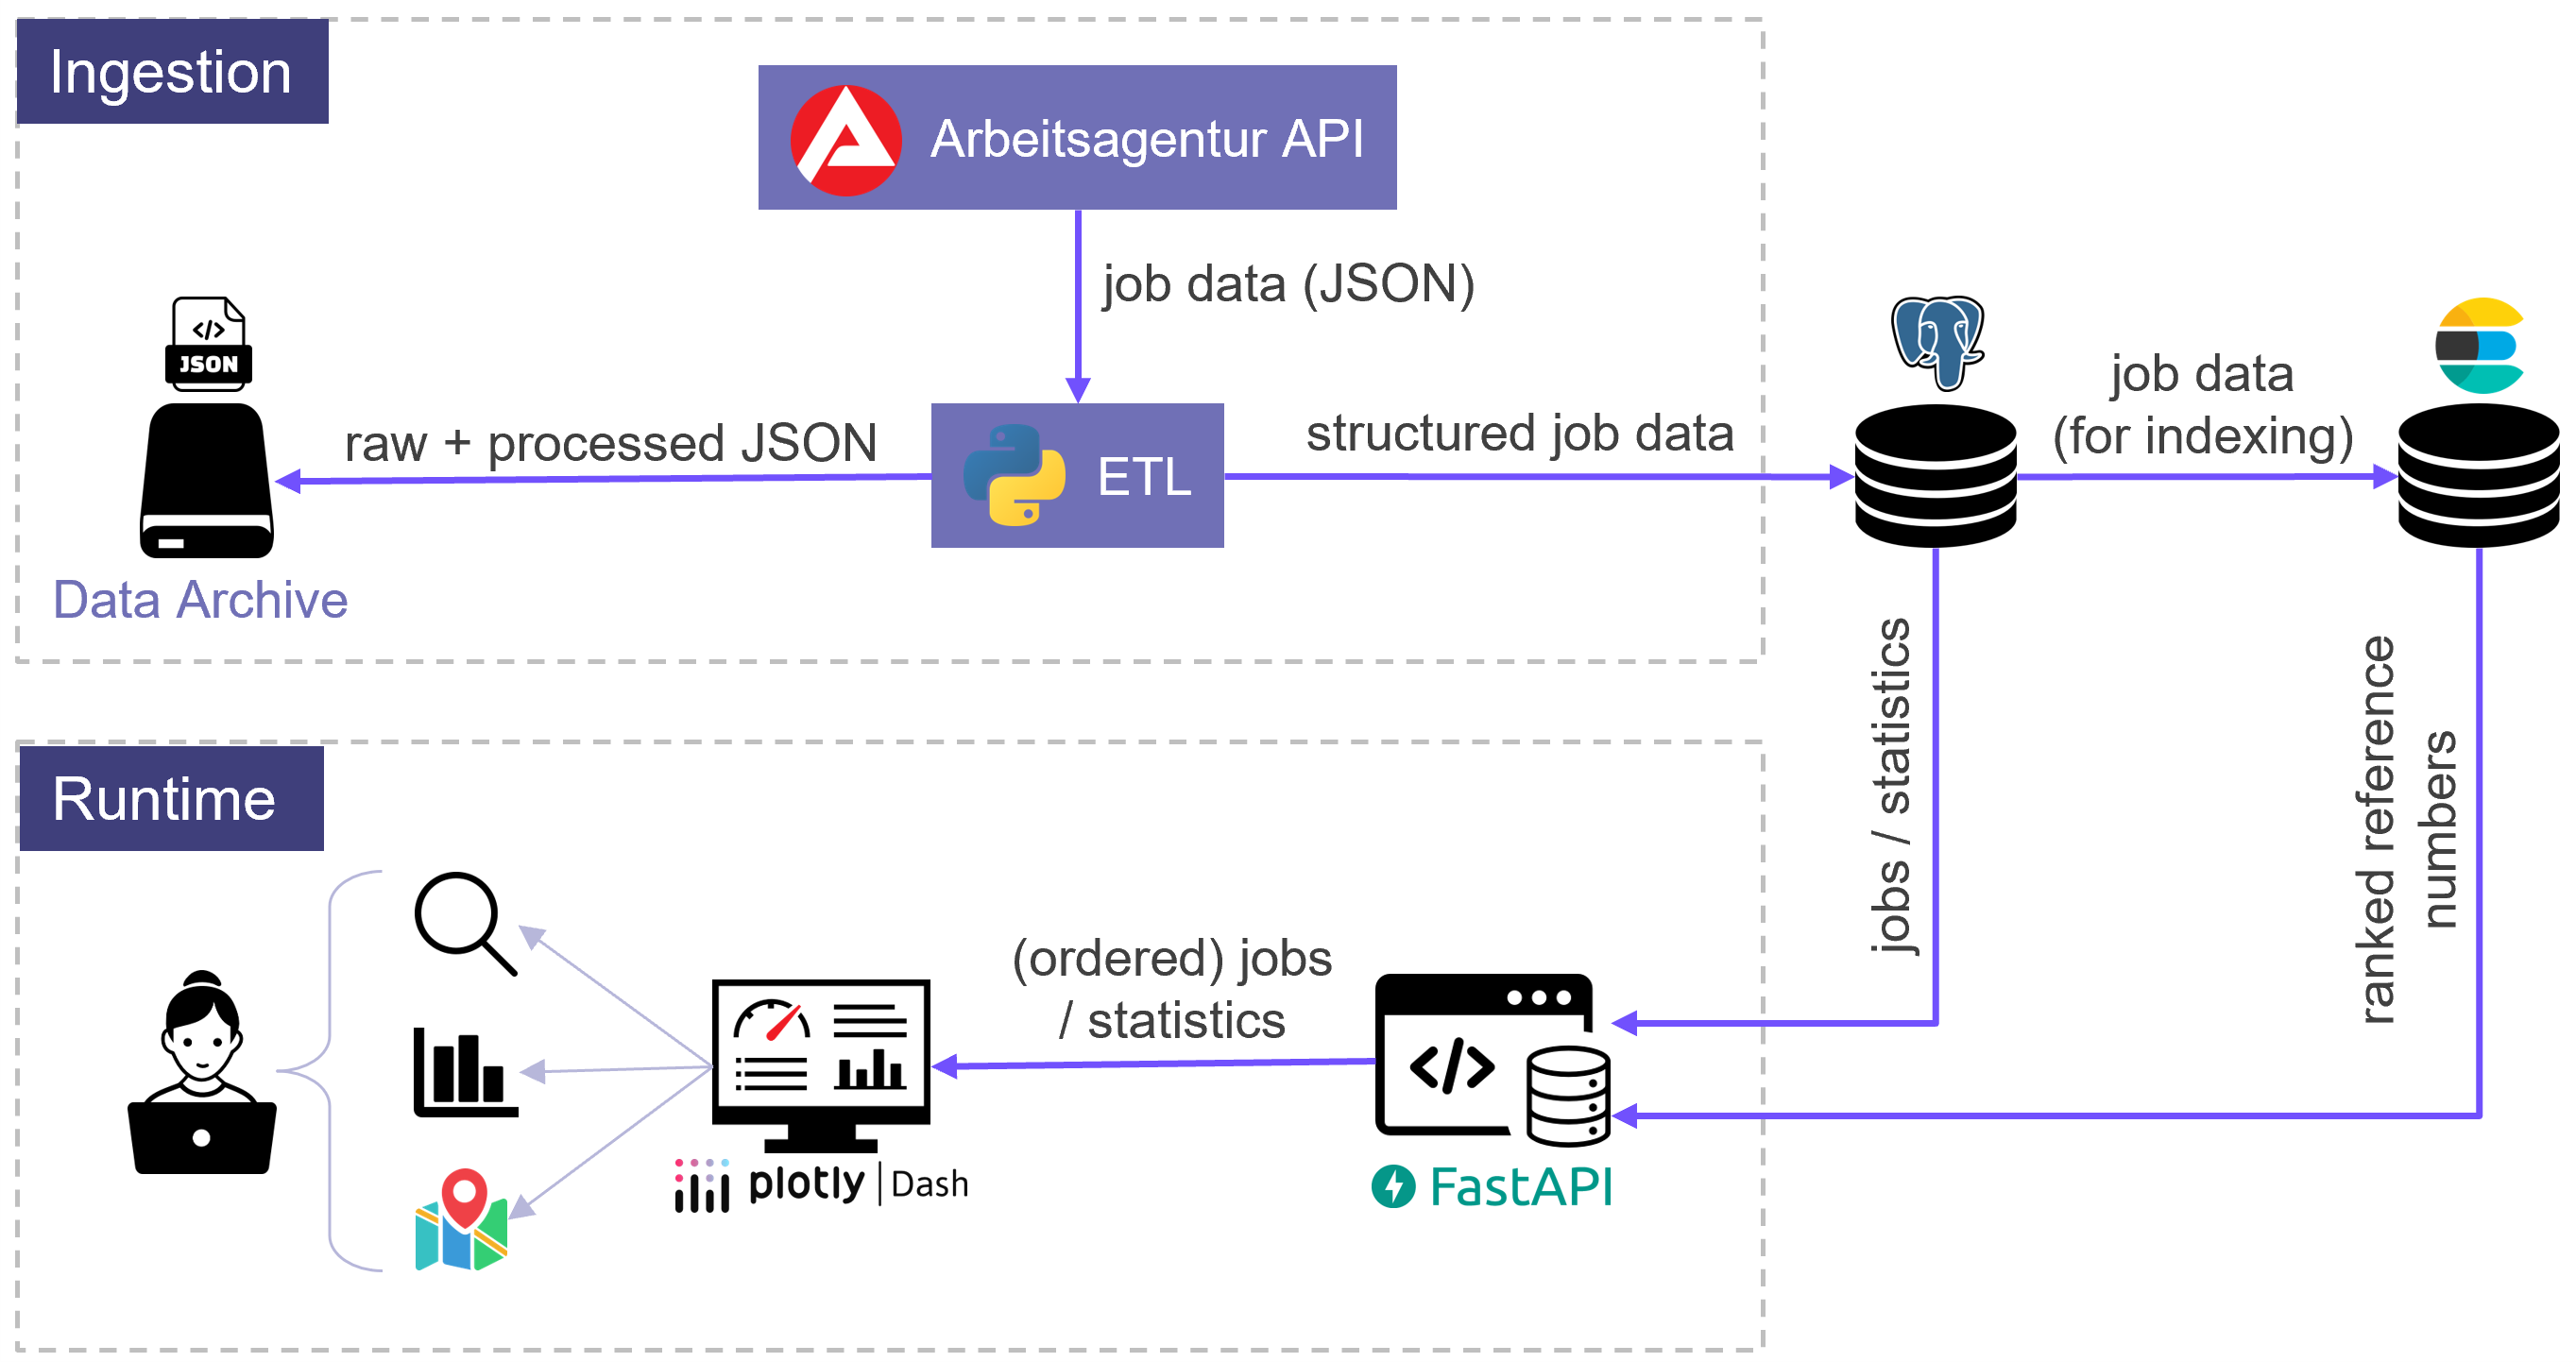
\includegraphics[width=0.85\textwidth,height=0.72\textheight,keepaspectratio]{project-overview.png}
	\caption{Overall architecture of the Job Market system.}
	\label{fig:project-overview}
\end{figure}

The ingestion side is centred on a Python ETL pipeline that retrieves job advertisements from the Bundesagentur für Arbeit API (\cite{arbeitsagentur-api}). The extraction stage preserves the original JSON responses, while the transformation stage converts the source-specific representation into the internal job model, performs enrichment and classification, and prepares the records for persistence. PostgreSQL serves as the authoritative structured data store for the application. After the database has been updated and job freshness has been evaluated, the active advertisements are synchronised to Elasticsearch. The Elasticsearch index therefore represents a rebuildable, search-oriented projection of the PostgreSQL data rather than an independent source of truth.

The runtime side follows a layered application architecture. FastAPI forms the service layer between the data stores and the user interface and exposes job listings, details, filters, and aggregated statistics through HTTP endpoints. Requests without a keyword are handled directly through PostgreSQL. When a keyword is supplied, FastAPI uses Elasticsearch for full-text search and relevance ranking. Elasticsearch returns the matching job IDs in ranked order, after which the corresponding job records are retrieved from PostgreSQL while preserving that order. The Dash frontend consumes these endpoints rather than accessing either data store directly.

Data collection is automated with Airflow (\cite{airflow-docs}), while Prometheus, Pushgateway, and Grafana (\cite{prometheus-docs,prometheus-pushgateway,grafana-docs}) provide operational monitoring of the application and ETL process. These supporting components are described in more detail in the following sections. All major services are executed as Docker containers and connected through Docker Compose, providing a reproducible local runtime environment.

Figure~\ref{fig:tech-stack} summarises the main technologies used in each functional part of the system.

\begin{figure}[htbp]
	\centering
	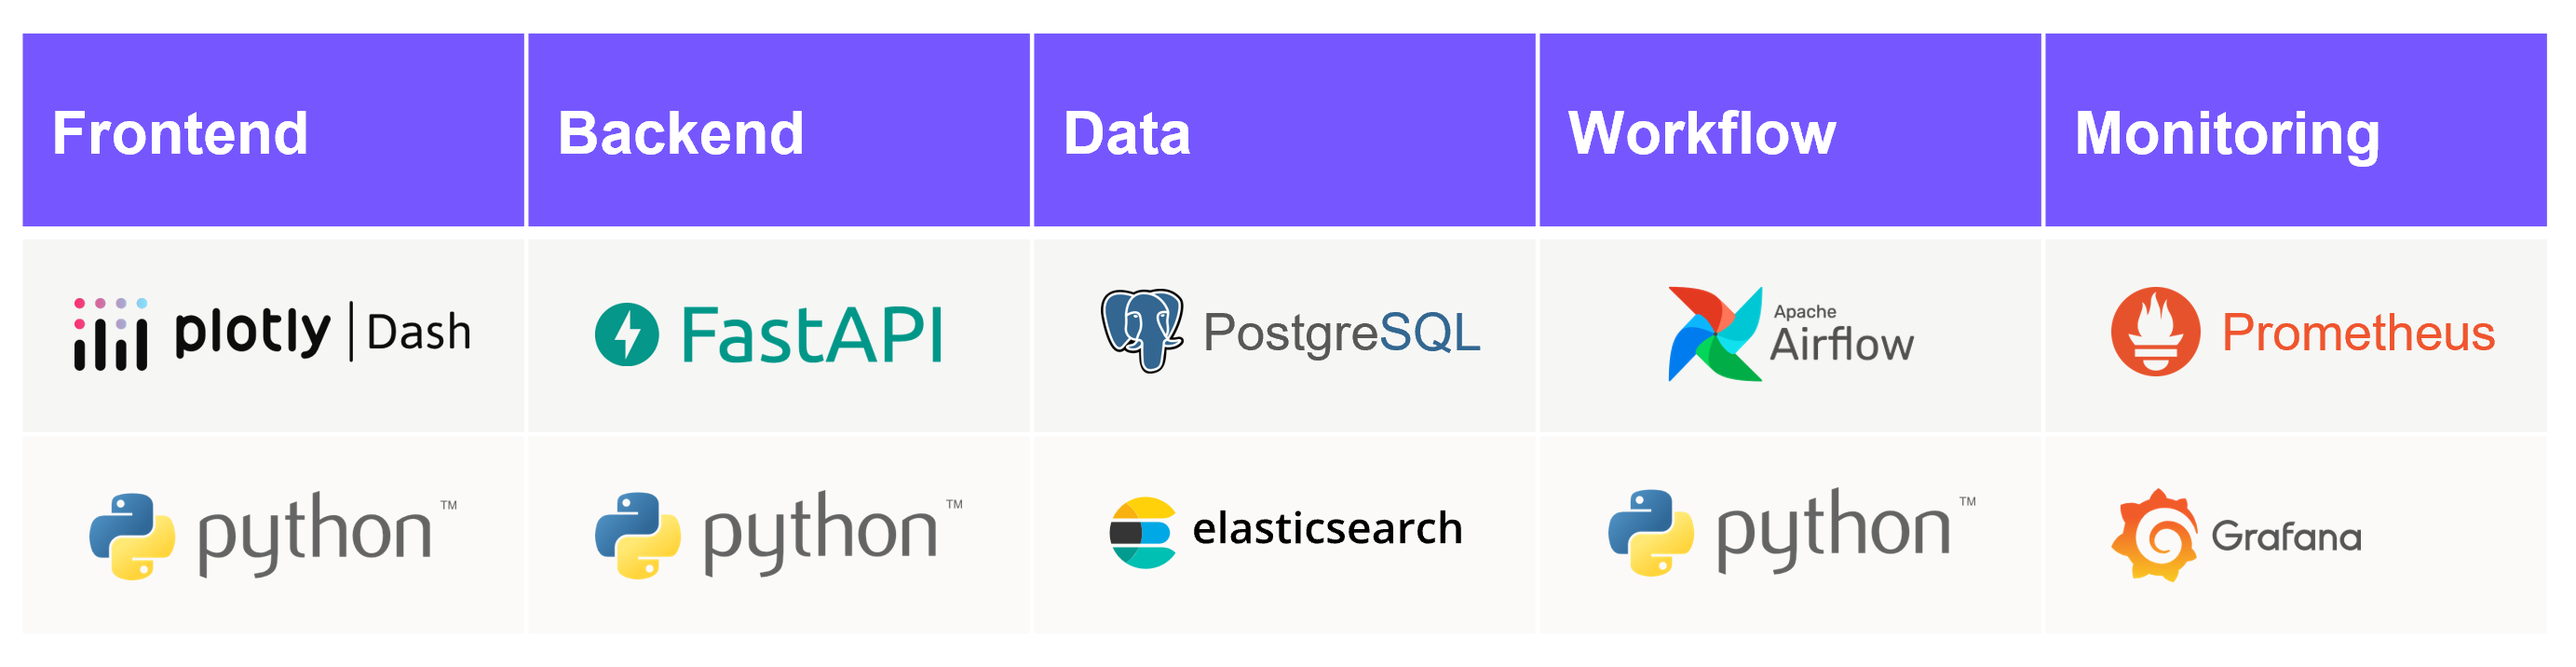
\includegraphics[width=0.85\textwidth]{tech-stack.png}
	\caption{Technology stack grouped by functional area.}
	\label{fig:tech-stack}
\end{figure}

The concrete flow of data through the ingestion pipeline, from API extraction to transformation, enrichment, persistence, and search-index synchronisation, is described in Section~\ref{sec:data-collection}.



\section{Data Collection and ETL Pipeline \label{sec:data-collection}}


\subsection{Data Source}

The project uses the job-search interface of the German Bundesagentur für Arbeit as its single data source. This choice matches the focus on the German labour market and provides structured job advertisements through HTTP endpoints without requiring the reconciliation of schemas from multiple providers. Alternatives such as Adzuna are subject to more restrictive request limits and potential licensing conditions, while The Muse is primarily oriented towards its own international job catalogue. Using a single consistent source therefore allowed the project to focus on the complete data-engineering workflow rather than on source-specific integration problems.

The API provides access to job advertisements in two stages. A keyword-based search first returns a list of matching job advertisements with their reference numbers. These \emph{reference numbers} can then be used to retrieve the complete \emph{details} of individual advertisements, as illustrated in Figure~\ref{fig:arbeitsagentur-api}.

\begin{figure}[htbp]
	\centering
	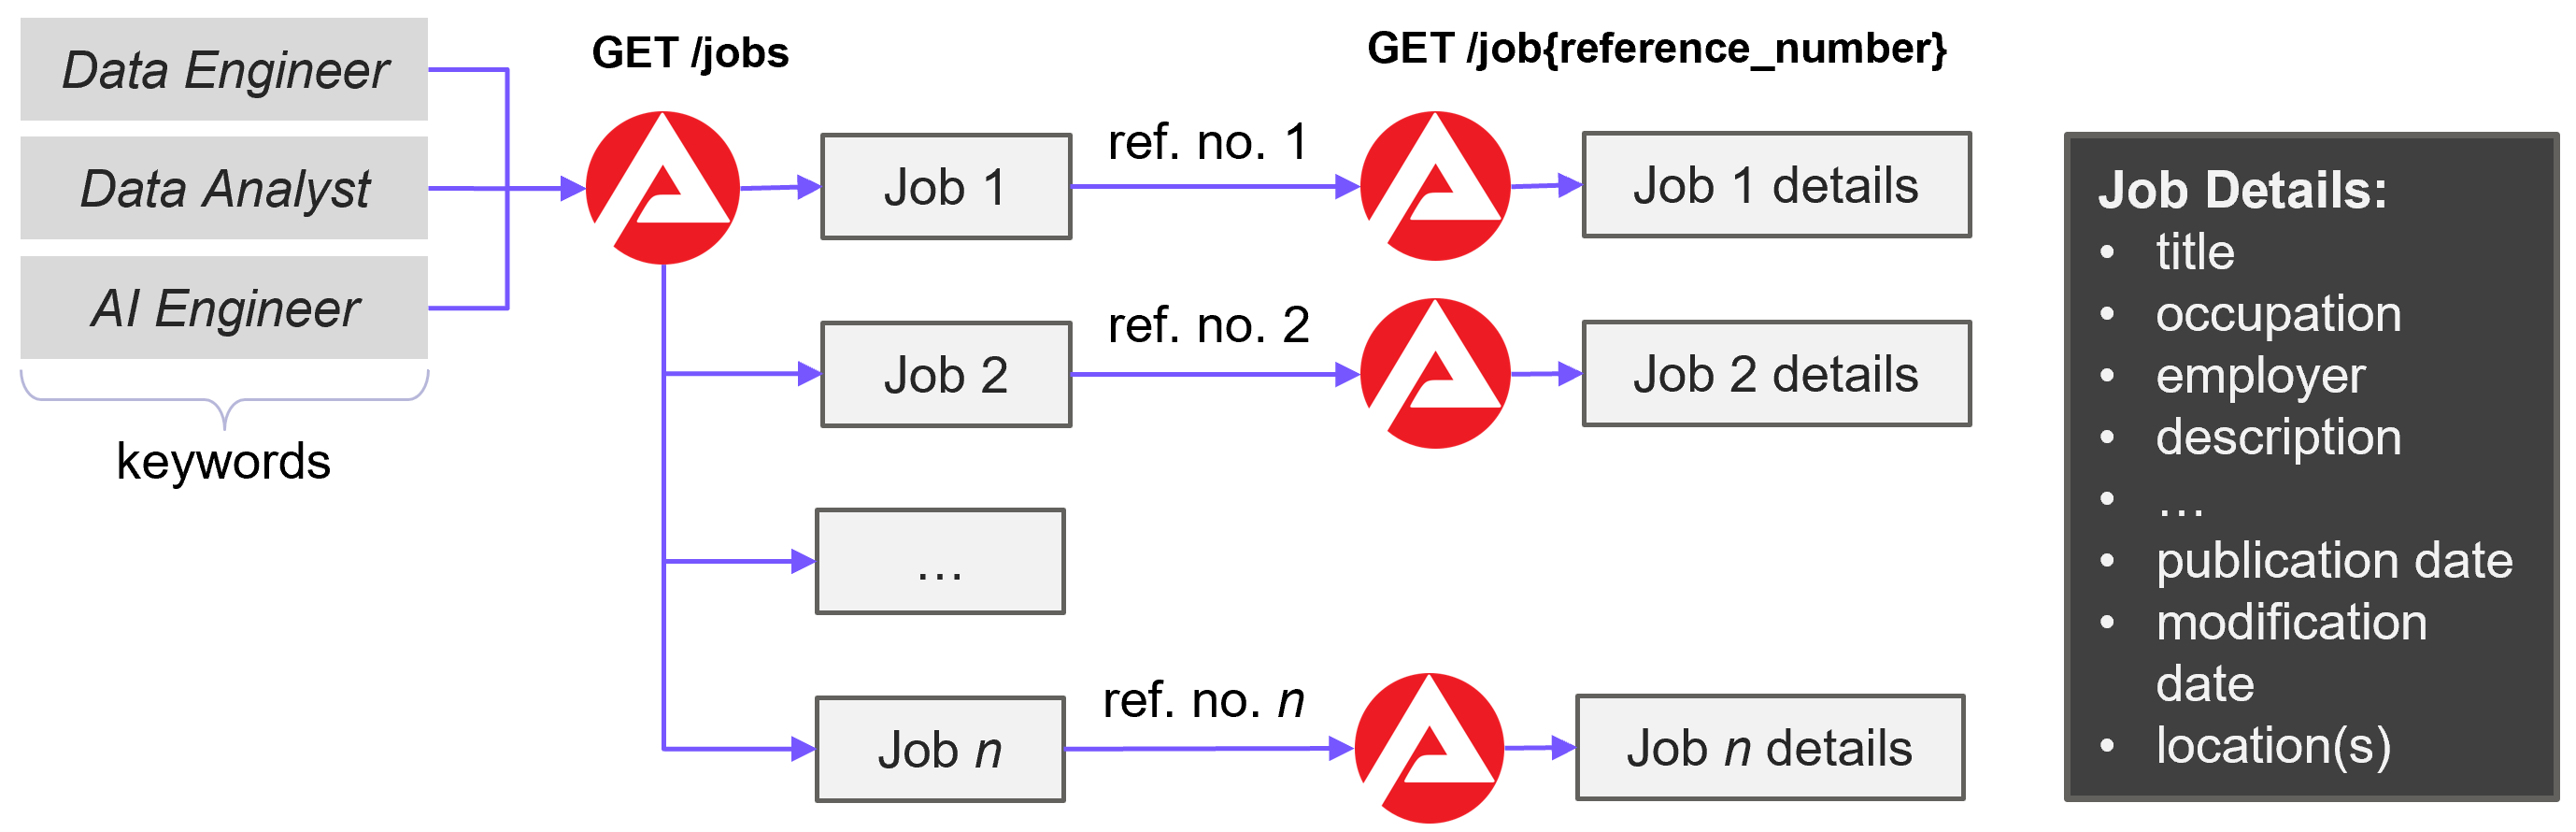
\includegraphics[width=0.85\textwidth]{arbeitsagentur-api.png}
	\caption{Two-stage retrieval of job advertisements from the Bundesagentur für Arbeit API: keyword-based search followed by detail retrieval using reference numbers.}
	\label{fig:arbeitsagentur-api}
\end{figure}

The job-search endpoint returns paginated advertisement lists and accepts a search keyword, an optional location, a page number, and a page size as parameters. The detail endpoint returns the complete advertisement record, including information such as title, occupation, employer, description, employment conditions, salary, publication and modification dates, external links, and one or more job locations.

A special case occurs when a previously observed advertisement is no longer available. If the detail endpoint returns HTTP 404 together with the source-specific code \path{STELLENANGEBOT_NICHT_GEFUNDEN}, this is interpreted as evidence that the advertisement no longer exists at the source. This distinction is important for job-freshness tracking because a confirmed disappearance must be distinguished from a temporary request failure.


\subsection{ETL Pipeline}

The ingestion process is divided into the three conventional ETL stages shown in Figure~\ref{fig:ingestion-pipeline}.

\begin{figure}[htbp]
	\centering
	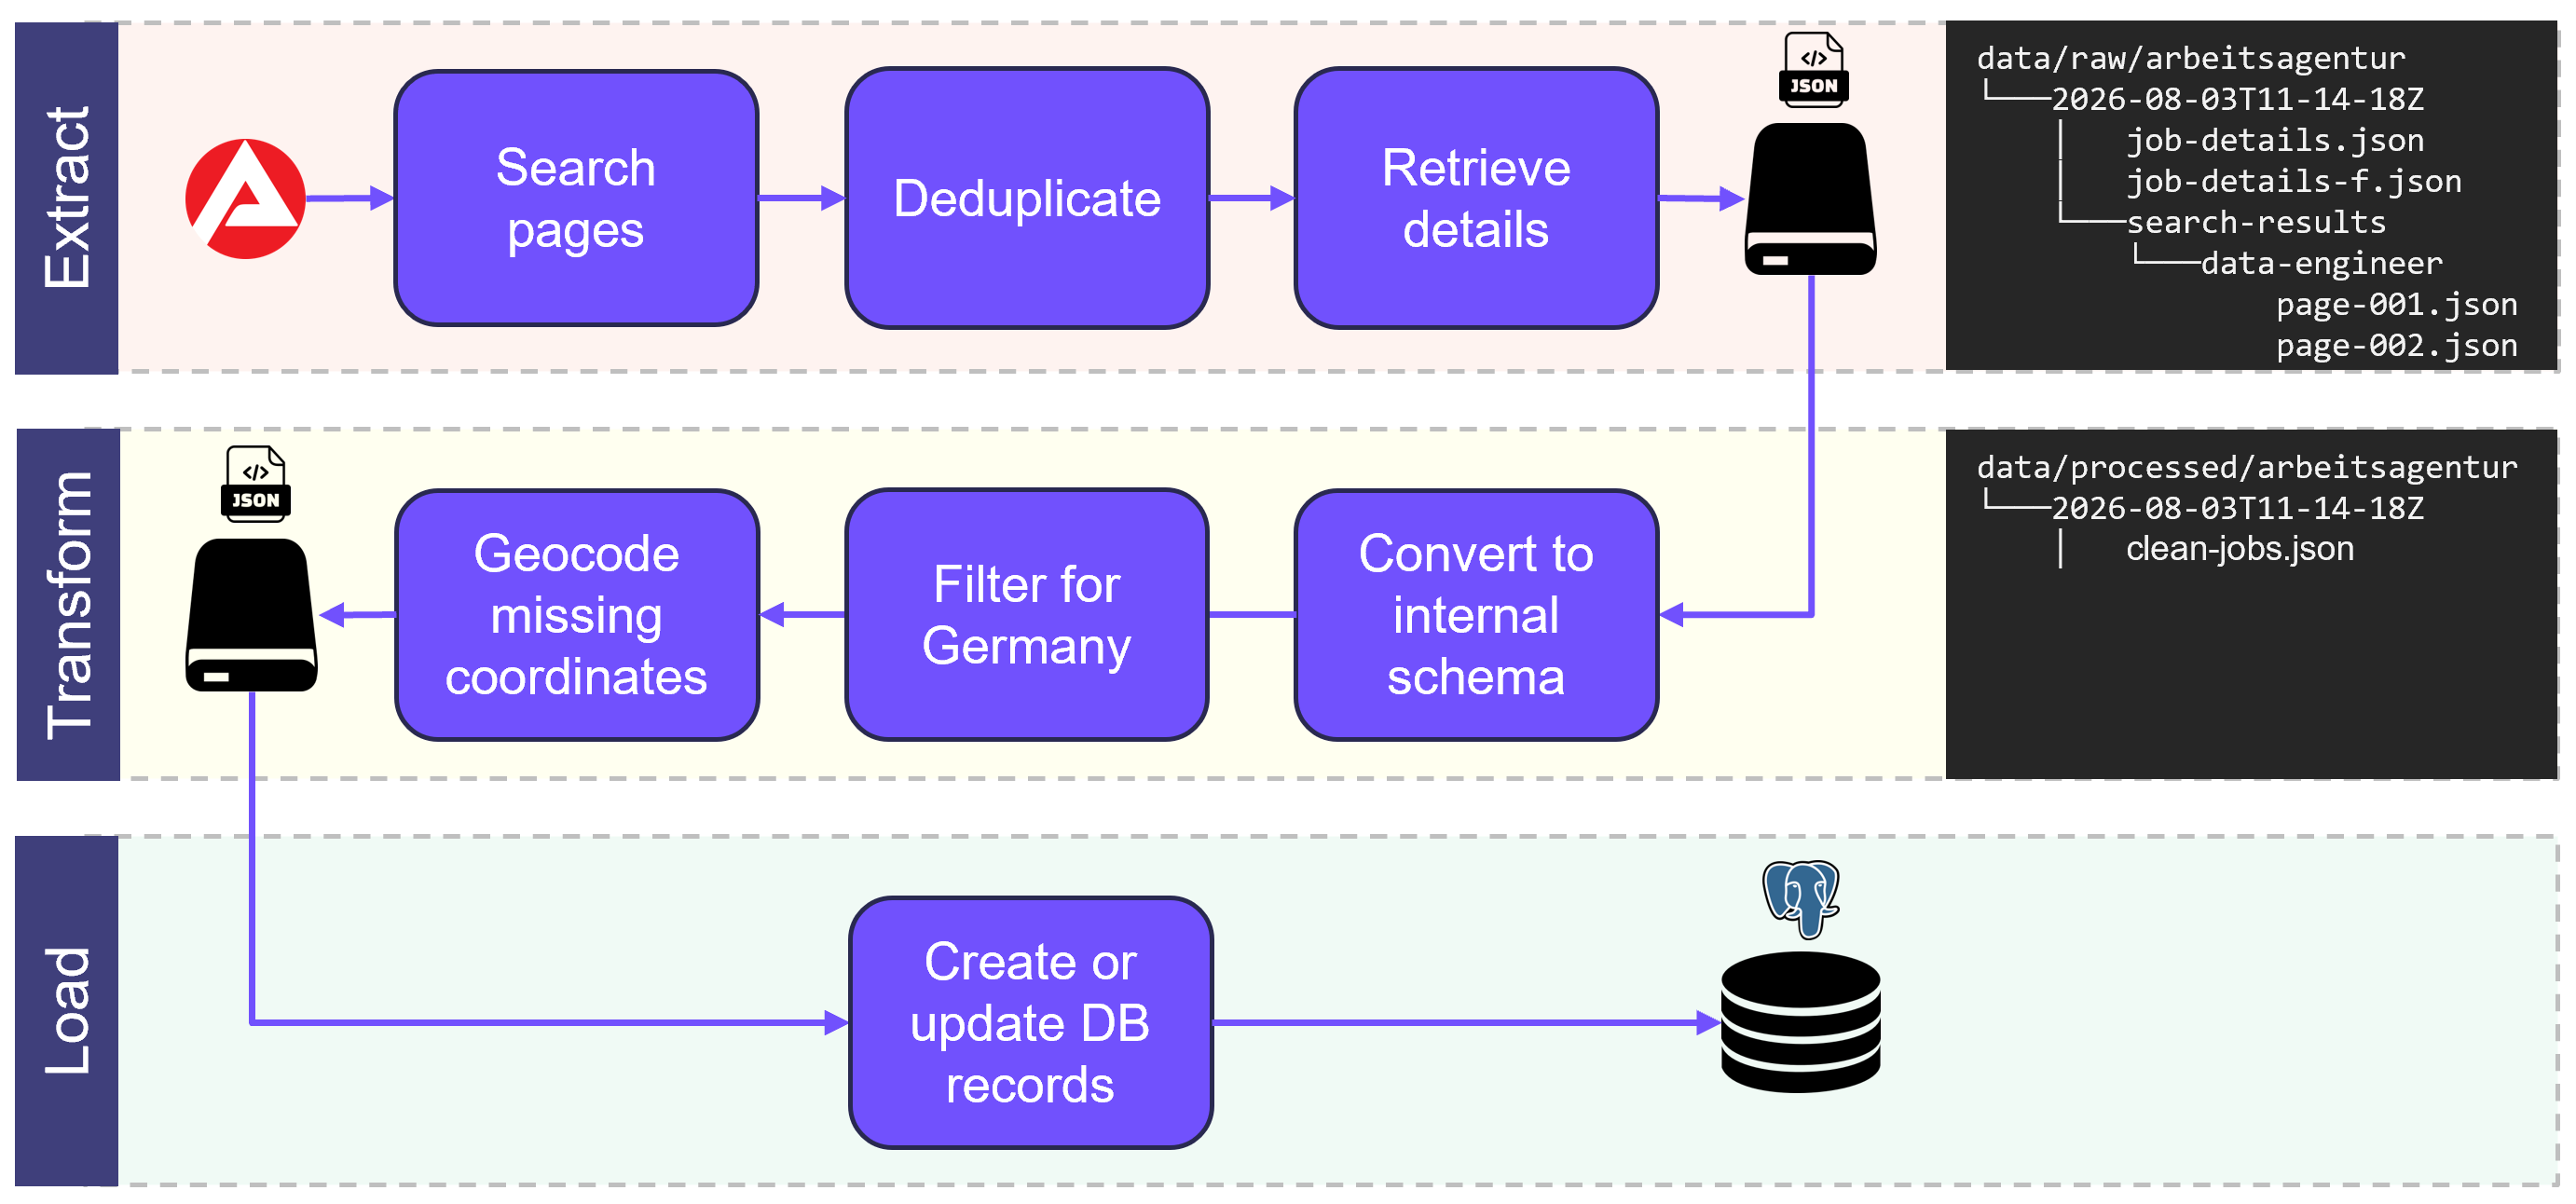
\includegraphics[
	width=0.85\textwidth,
	height=0.75\textheight,
	keepaspectratio
	]{ingestion.png}
	\caption{Extract, transform, and load stages of the ingestion pipeline.}
	\label{fig:ingestion-pipeline}
\end{figure}


\subsubsection{Extraction}

The extraction process is shown in the upper row of Figure~\ref{fig:ingestion-pipeline}.

An extraction run can process several search keywords. For each keyword, the first search-result page is requested and its pagination metadata is used to determine the total number of pages. The API reports the maximum number of results and the effective page size, from which the extraction code calculates the required number of requests. Every successfully retrieved page is preserved unchanged as JSON under a keyword-specific directory. This creates a raw archive of the actual search responses rather than retaining only the subsequently transformed records.

The same advertisement may occur in the result sets of several search terms. Reference numbers are therefore deduplicated across all keywords within an extraction run to avoid unnecessary processing. Malformed result entries and advertisements without a valid reference number are skipped. The resulting set of unique references represents the jobs observed during the current search and is also retained for the subsequent job-freshness update.

As noted above, the API exposes job advertisements in two stages: search requests return summary information together with a unique reference number, while the complete advertisement must be retrieved separately using that reference number. Full job details are therefore retrieved using the unique reference numbers obtained from the search results. To reduce unnecessary API requests, an existing advertisement is not automatically downloaded again on every run. The extraction code compares the source modification timestamp, \path{aenderungsdatum}, with the timestamp already stored for that job. Detail retrieval is required for new advertisements, advertisements whose modification timestamp has changed, and cases in which the timestamps are missing or cannot be compared reliably. Unchanged advertisements can therefore remain in PostgreSQL without repeatedly downloading and processing identical detail records.

A failure to retrieve an individual detail record does not abort the complete extraction. Successful responses are collected in \path{job-details.json}, while failed requests are written separately to \path{job-detail-failures.json} together with the affected reference number and error message. The remaining advertisements can therefore continue through the pipeline, while failed requests remain traceable for diagnosis.

Each extraction run receives its own UTC-timestamped directory under \path{data/raw/arbeitsagentur}. Within this directory, the individual search-result pages are stored under \path{search-results/<keyword>/}, while retrieved detail records and detail-request failures are stored at the run level. For example, a run may create a directory such as \path{data/raw/arbeitsagentur/2026-08-03T11-14-18Z/}. Keeping each run separate preserves the original source data and provides a reproducible record of what was returned by the external service at a particular point in time.


\subsubsection{Transformation}

The transformation stage converts the source-specific JSON representation returned by the Bundesagentur für Arbeit into the internal schema used by the remainder of the application. As shown in Figure~\ref{fig:ingestion-pipeline}, it is positioned between the raw JSON archive and PostgreSQL persistence and produces a cleaned and enriched intermediate dataset.

German field names from the source API are mapped to consistent English names, for example \path{referenznummer} to \path{reference_number}, \path{stellenangebotsTitel} to \path{title}, and \path{firma} to \path{company}. The same principle is applied to employment conditions, salary information, dates, external links, and employer metadata. This isolates the rest of the application from the terminology and structure of the external API and provides a stable internal representation for persistence and consumption.

Nested structures are normalised during the same process. The source field \path{stellenlokationen} may contain several job locations, which are converted into a list of location objects containing postal code, city, region, country, latitude, and longitude. Entry and publication periods are similarly reduced to the relevant start dates used by the internal model. The transformation is designed to tolerate incomplete or malformed source data: missing optional fields become null values, while malformed nested structures or individual location entries are ignored rather than causing the entire transformation to fail.

After structural normalisation, only advertisements containing at least one location in \path{DEUTSCHLAND} are retained. Each job is assigned one of the project's standardised categories based on its title and occupation, and missing geographic coordinates are enriched by the location geocoder. Malformed locations encountered during geocoding are counted and reported by the transformation process.

The transformed records are written to \path{clean-jobs.json} under \path{data/processed/arbeitsagentur/<timestamp>/}, using the timestamp inherited from the corresponding extraction run. The archived source responses remain unchanged, preserving a clear distinction between immutable raw input and the cleaned data consumed by the loading stage.

\paragraph{Location Enrichment}

Job advertisements may already contain geographic coordinates for their locations. When both latitude and longitude are available from the source, these values are retained unchanged and the location is marked with \path{coordinates_source = "source"}. Only locations with missing coordinates are passed to the additional geocoding step shown in Figure~\ref{fig:ingestion-pipeline}.

Missing coordinates are resolved using the Nominatim geocoding service (\cite{nominatim-api}) through the \path{geopy} library. A query is constructed from the available postal code, city, and country fields. Successful results are stored with \path{coordinates_source = "geocoded"}, while unsuccessful lookups leave the coordinates empty and mark the source as \path{"missing"}. Requests are passed through \texttt{geopy}'s \texttt{RateLimiter} to comply with the Nominatim usage policy \cite{nominatim-policy}. The geocoder is configured to enforce a minimum delay of one second between requests and to retry temporary failures.

To avoid repeated external requests, the geocoder maintains an in-memory cache indexed by the normalised location query. Both successful and unsuccessful lookups are cached, so multiple advertisements referring to the same postal code, city, and country combination normally require only one Nominatim request during an ETL run.


\paragraph{Job Classification \label{sec:job-classification}}

To support filtering and statistical analysis, each transformed advertisement is assigned to one of the broad job categories shown in Figure~\ref{fig:job-classification}. The categories are deliberately broader than individual job titles so that advertisements with different naming conventions can be compared at an aggregate level. Jobs that do not match any configured category are assigned to \textit{Other}.

\begin{figure}[htbp]
	\centering
	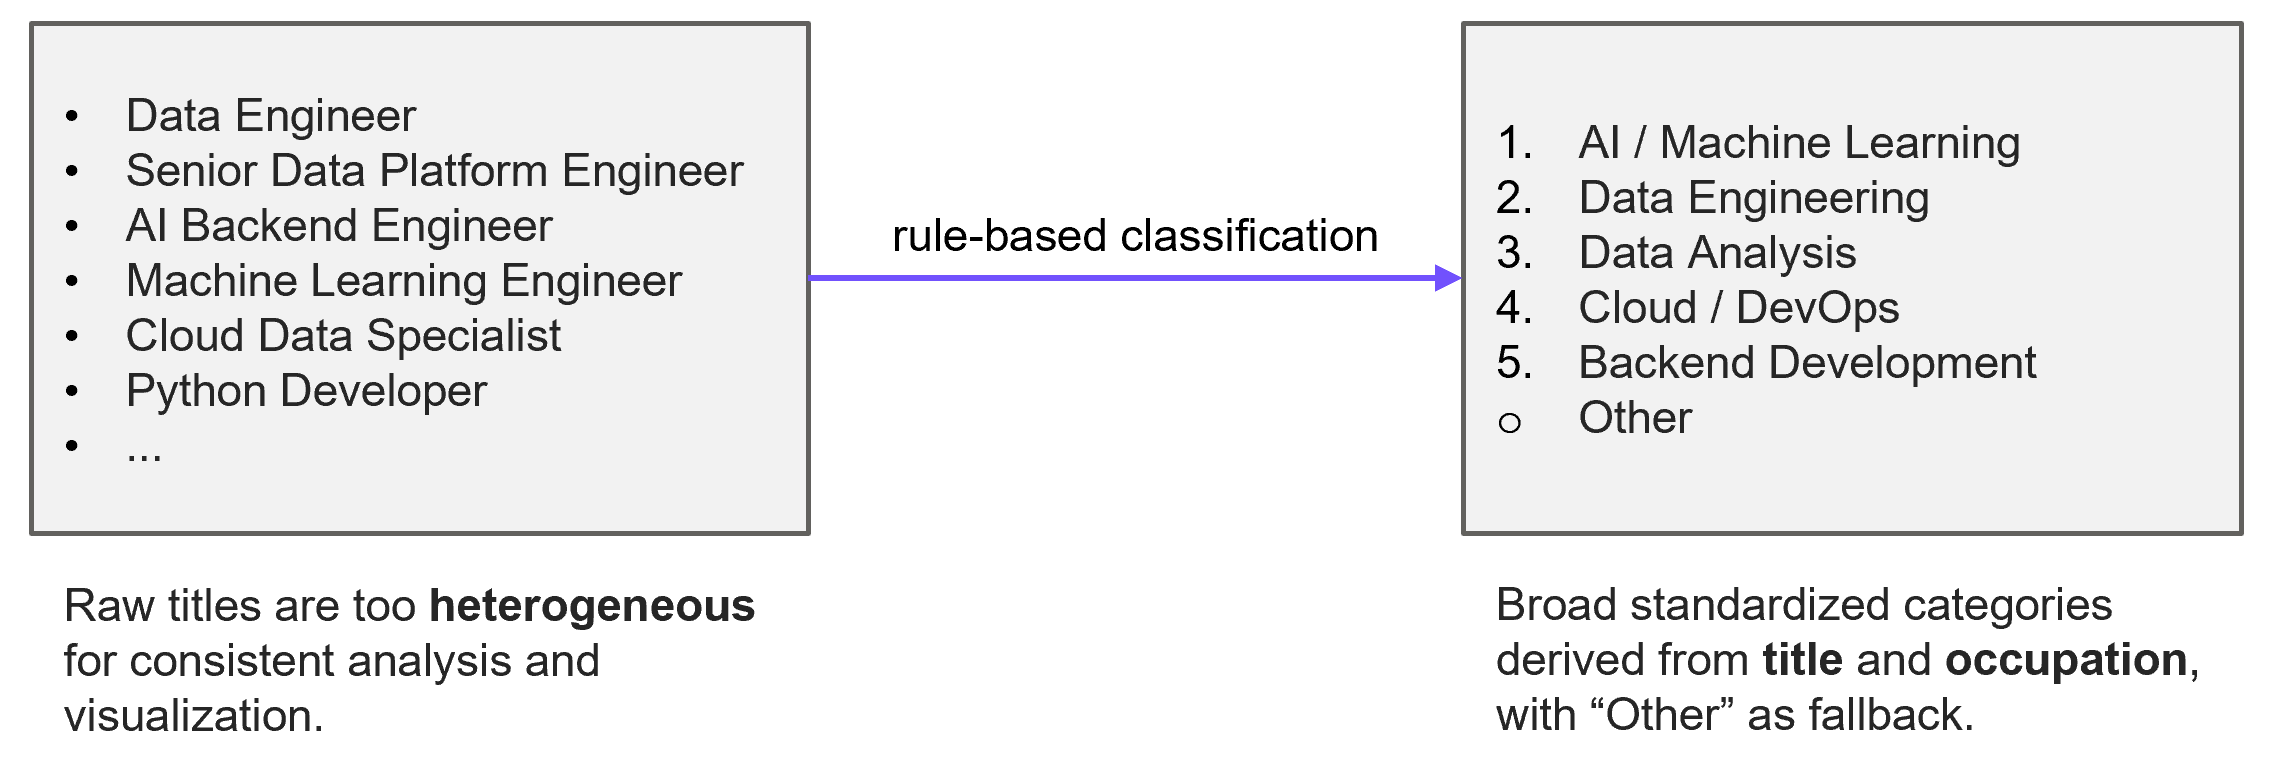
\includegraphics[
	width=\textwidth,
	keepaspectratio
	]{classification.png}
	\caption{Rule-based standardisation of heterogeneous job titles into broad job categories.}
	\label{fig:job-classification}
\end{figure}

Classification is performed during the transformation stage shown in Figure~\ref{fig:ingestion-pipeline}. The classifier combines the job title and occupation fields, normalises the resulting text, and compares it with predefined category-specific keyword lists.

Because an advertisement may contain terms associated with several categories, classification follows a fixed priority order (Figure~\ref{fig:job-classification}, right box). The first match determines the category. For example, a position titled \textit{Backend Developer for Machine Learning} is classified as \textit{AI / Machine Learning} rather than \textit{Backend Development}. This keeps the classification deterministic while resolving common ambiguities.

Short keywords require special handling because simple substring matching can produce false positives when an abbreviation occurs inside a longer word. Keywords of three characters or fewer are therefore matched as complete terms using regular-expression boundaries. This applies, for example, to abbreviations such as \texttt{ETL}, \texttt{NLP}, \texttt{LLM}, and \texttt{SRE}.

The approach is intentionally lightweight and transparent, but depends entirely on the configured keywords and the wording of the title and occupation fields. Unrepresented synonyms or uncommon titles may therefore be assigned to \textit{Other}, while advertisements spanning several disciplines are reduced to a single category according to the fixed priority. The resulting categories are suitable for broad exploration and visualisation but should not be interpreted as a formal occupational classification.


\subsubsection{Loading \label{sec:loading}}

The loading stage persists the cleaned records produced by the transformation stage into PostgreSQL and completes the ETL process shown in Figure~\ref{fig:ingestion-pipeline}.

Before loading, the required relational schema is created if it does not yet exist. The main \texttt{jobs} table stores the advertisement data, while locations are normalised into the separate \path{job_locations} table because one advertisement may refer to multiple locations.

The reference number supplied by the Bundesagentur für Arbeit is used as the stable identifier of an advertisement and forms the primary key of the \texttt{jobs} table. Date-like values such as publication and modification timestamps are converted into values compatible with the corresponding PostgreSQL column types before insertion.

Jobs are persisted using PostgreSQL's \texttt{INSERT ... ON CONFLICT ON UPDATE} mechanism. A previously unseen reference number creates a new row, while an existing reference number causes the stored advertisement to be updated with the latest source data. Re-running the pipeline therefore does not create duplicate advertisements: the same source advertisement continues to correspond to one database row.


\paragraph{Update Strategy}

In addition to the current advertisement data, the loader distinguishes genuine modifications from unchanged republications. A newer \path{publication_date} does not necessarily indicate a changed advertisement, because a job may be republished while its \path{modified_at} value remains unchanged. Figure~\ref{fig:job-freshness} illustrates how these cases are distinguished during freshness tracking.

\begin{figure}[htbp]
	\centering
	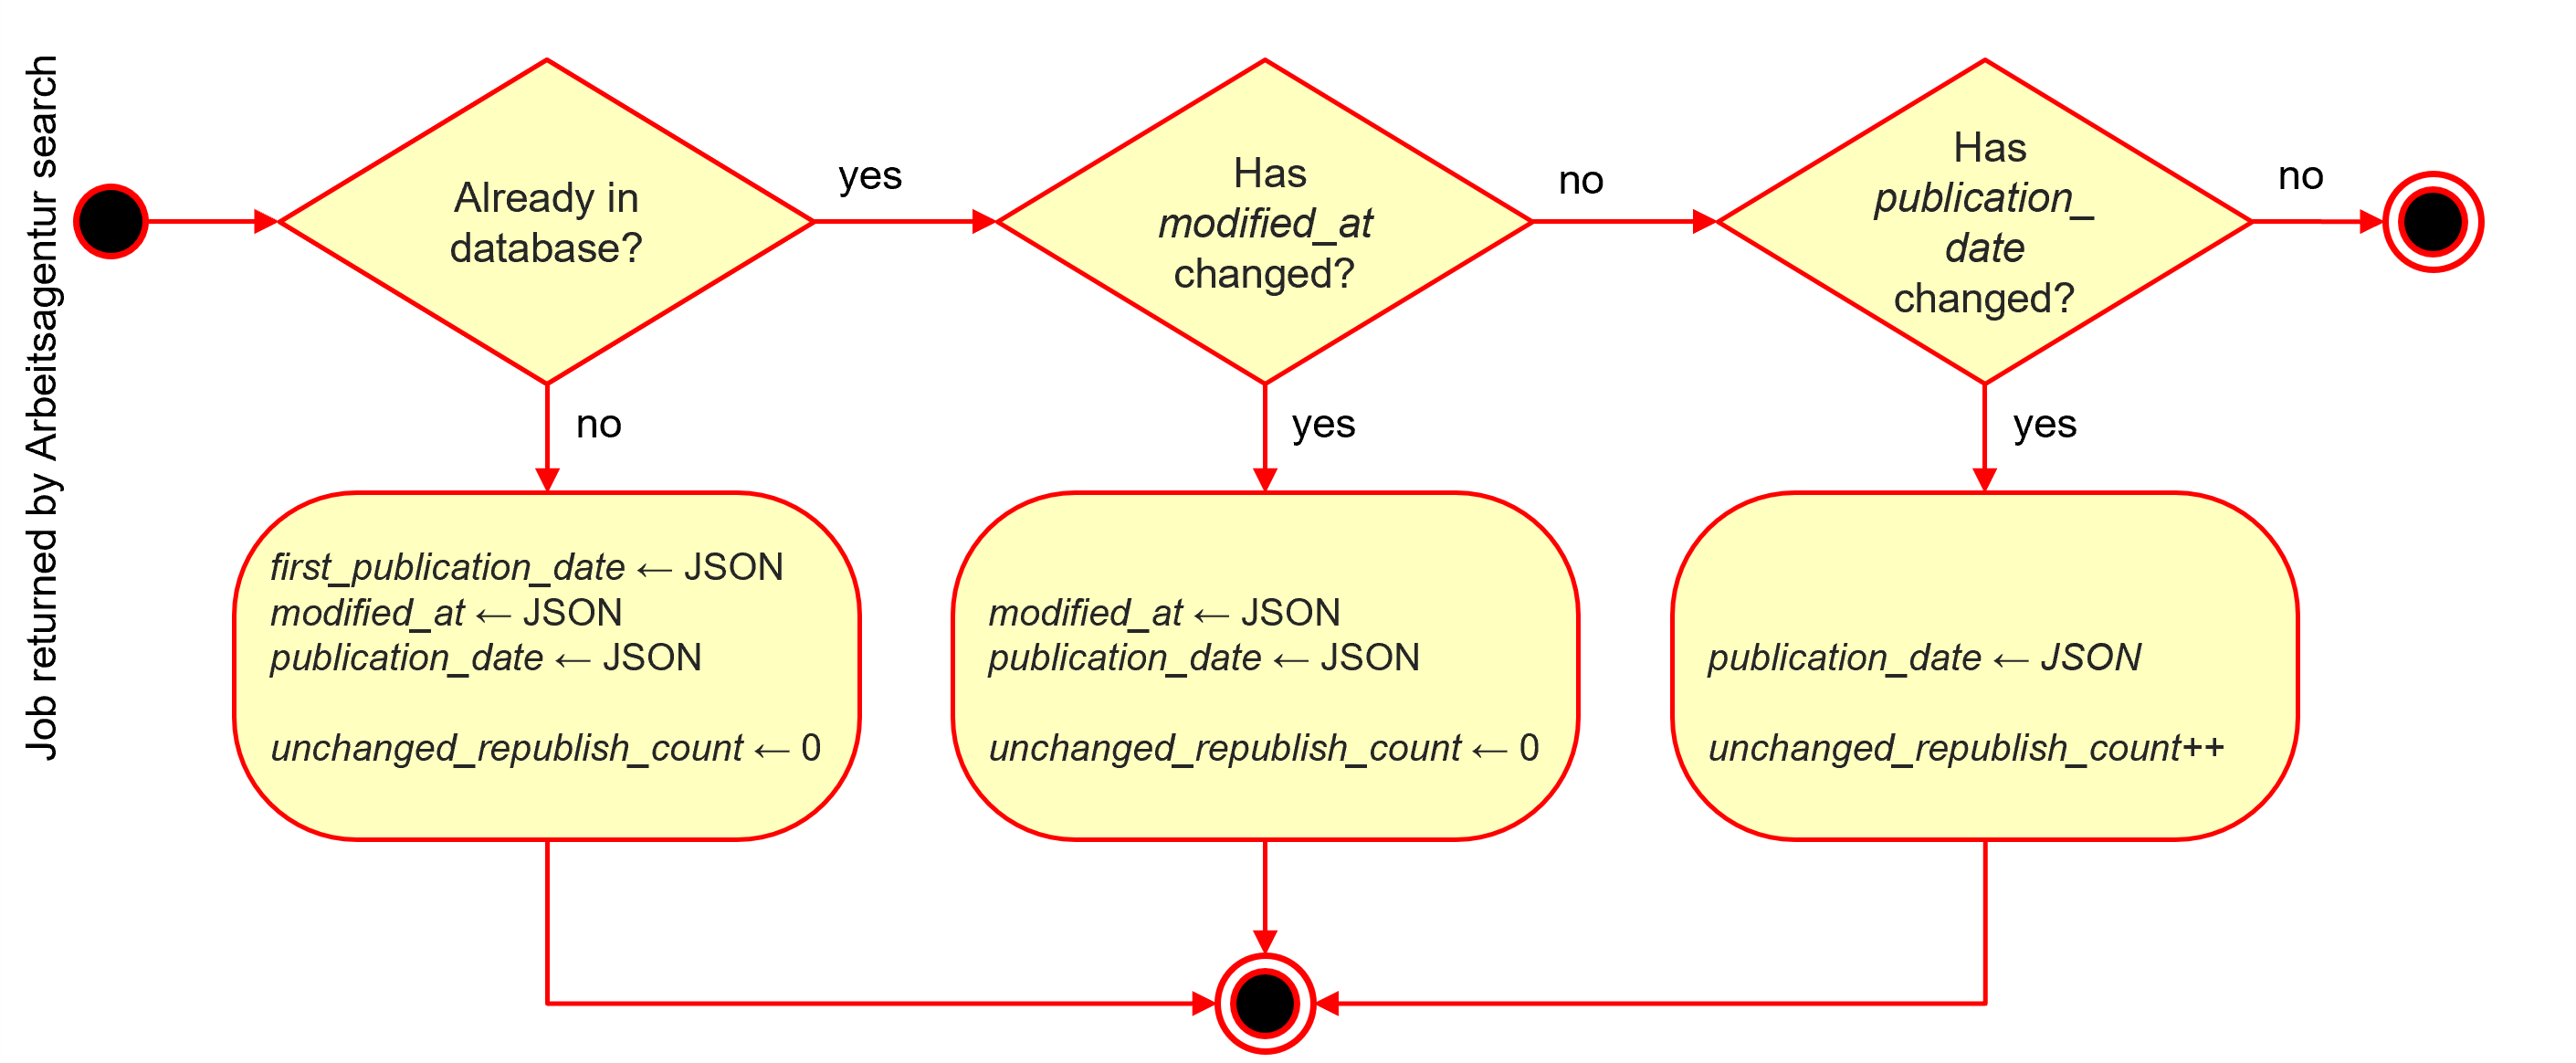
\includegraphics[
	width=\textwidth,
	keepaspectratio
	]{job-freshness.png}
	\caption{Detection of job modifications and unchanged republications.}
	\label{fig:job-freshness}
\end{figure}

A changed \path{modified_at} value is interpreted as a genuine modification. If \path{modified_at} remains unchanged while \path{publication_date} changes, the advertisement is treated as an unchanged republication and \path{unchanged_republish_count} is incremented. The original \path{first_publication_date} is retained as the earliest publication date observed by the project.

After a job is inserted or updated, its stored locations are replaced by those in the current cleaned record. Each location is linked to the job through a foreign key with \texttt{ON DELETE CASCADE}, ensuring that associated location records are removed automatically if the parent job is deleted.

The job update and location replacement are performed within a database transaction: if part of the operation fails, the transaction is rolled back, preventing partially updated advertisements. Invalid records are logged and skipped while processing continues with the remaining jobs.


\subsection{Elasticsearch Index Synchronisation \label{subsec:elasticsearch-index-sync}}

Elasticsearch is maintained as a derived search index rather than as an independent data store. PostgreSQL remains the authoritative source of job data, and the Elasticsearch index is rebuilt from the current database state after each scheduled ETL run. In the Airflow workflow, database loading and the job-freshness update are completed before Elasticsearch synchronisation, ensuring that the index reflects the latest active state of the advertisements.

During synchronisation, all active jobs are selected from PostgreSQL together with the fields required for full-text search and filtering, as listed in Table~\ref{tab:elasticsearch-mapping}. Because a single job may be associated with several rows in the \path{job_locations} table, the distinct city names from these rows are collected into a single \path{cities} array in the Elasticsearch document. For example, a job with locations in Berlin and Potsdam is represented with \path{cities = ["Berlin", "Potsdam"]}. One Elasticsearch document therefore represents one job advertisement regardless of how many locations are stored for it in PostgreSQL.

For each synchronisation, the existing jobs index is recreated and populated with the selected advertisements. The job's unique \path{reference_number}, which serves as the primary key in PostgreSQL, is also used as the Elasticsearch document identifier. This keeps the same job directly identifiable in both data stores. Table~\ref{tab:elasticsearch-mapping} summarises the Elasticsearch field mapping and shows how the selected attributes are indexed.

\begin{table}[htbp]
	\centering
	\begin{tabular}{lll}
		\hline
		\textbf{Field} & \textbf{Elasticsearch type} & \textbf{Purpose} \\
		\hline
		\texttt{reference\_number}     & \texttt{keyword}        & stable job identifier \\
		\texttt{title}                 & \texttt{text}           & full-text search \\
		\texttt{occupation}            & \texttt{text}           & full-text search \\
		\texttt{description}           & \texttt{text}           & full-text search \\
		\texttt{company}               & \texttt{text + keyword} & search and exact representation \\
		\texttt{category}              & \texttt{text + keyword} & search and exact filtering \\
		\texttt{cities}                & \texttt{keyword}        & exact city filtering \\
		\texttt{home\_office\_possible}& \texttt{boolean}        & boolean filtering \\
		\texttt{is\_active}            & \texttt{boolean}        & active-job filtering \\
		\hline
	\end{tabular}
	\caption{Elasticsearch mapping for searchable job advertisements.}
	\label{tab:elasticsearch-mapping}
\end{table}

Fields mapped as \texttt{text} are analysed for full-text queries, whereas \texttt{keyword} fields retain exact values for filtering. Multi-fields are used for \texttt{company} and \texttt{category}, allowing the same value to support both use cases. Lowercase normalisation is applied where case-insensitive exact filtering is required.

Because the index is a rebuildable projection of PostgreSQL, it can be discarded and recreated without loss of application data. Rebuilding it from active jobs also ensures that advertisements no longer considered active are removed from the search index.




\section{Data Modelling and Storage}


\subsection{Storage Strategy}

The project uses a two-layer storage strategy. Raw API responses are preserved unchanged in timestamped JSON directories, providing a lightweight historical archive of individual extraction runs. This makes the source data traceable and allows transformations to be reproduced without introducing the infrastructure and operational complexity of a dedicated data lake. The cleaned JSON produced during transformation serves only as an intermediate ETL artifact.

PostgreSQL stores the transformed application data because job advertisements and locations form a stable relational structure that is frequently filtered, joined, and aggregated. It provides referential integrity, transactions, indexing, and efficient SQL-based analysis, while SQLAlchemy (\cite{sqlalchemy-docs}) is used as the Python database-access layer for executing queries and managing connections.

A document database such as MongoDB could store the nested source responses directly, but provides little advantage after transformation into the stable relational schema. Preserving the original responses as JSON while storing the structured representation in PostgreSQL therefore provides the required flexibility without operating an additional database system.


\subsection{Relational Data Model}

The transformed data is represented by two related tables. The \texttt{jobs} table stores the attributes of a job advertisement and uses the source reference number as its primary key. The \path{job_locations} table stores geographical information and references the corresponding advertisement through a foreign key. A job may therefore have zero or more locations, while each location belongs to exactly one job.

\begin{figure}[htbp]
	\centering
	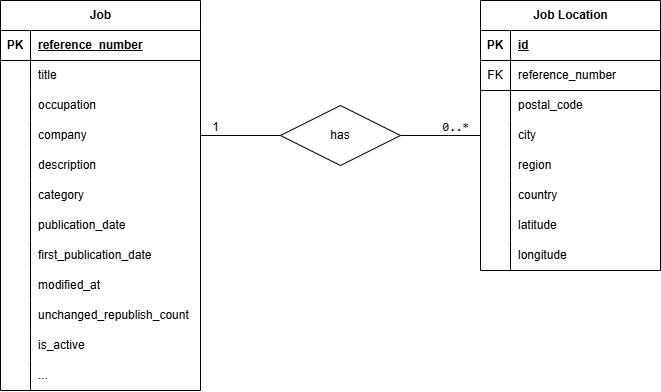
\includegraphics[width=0.72\textwidth, height=0.72\textheight, keepaspectratio]{erd.png}
	\caption{Entity--relationship diagram of the job-market database}
	\label{fig:erd}
\end{figure}

Separating jobs and locations avoids duplicating the complete advertisement when a job is associated with several locations. The foreign-key constraint preserves referential integrity, while \texttt{ON DELETE CASCADE} removes dependent locations when a job is deleted. A dedicated index is created on \path{job_locations.reference_number} to support efficient retrieval and joins by advertisement.

Most source-derived attributes are nullable because the API does not provide all information for every advertisement. Application-controlled values, such as the standardised category and freshness state, use defined defaults instead. The source reference number uniquely identifies advertisements and, together with PostgreSQL's \texttt{INSERT ... ON CONFLICT DO UPDATE}, prevents duplicate job rows during repeated ETL runs.




\section{Data Access and Visualisation}


\subsection{FastAPI Backend}

FastAPI was selected as the service layer between PostgreSQL and the user-facing dashboard. It provides a lightweight Python framework that integrates naturally with the rest of the application and supports typed request and response contracts. Query parameters such as pagination values and optional job filters are validated automatically, while Pydantic response models provide a stable JSON representation independently of the underlying SQL query results.

The Pydantic models are also used by FastAPI to generate the OpenAPI specification and interactive Swagger documentation. When the backend is running, the available endpoints can be inspected and tested directly through \path{http://127.0.0.1:8000/docs}. This provides a convenient way to verify API requests and responses independently of the frontend.

The API also establishes a clear boundary between data access and presentation. PostgreSQL is accessed only through the backend, while the Dash frontend communicates with FastAPI through HTTP and renders the returned JSON data. Database queries, filtering, validation, and statistical aggregation therefore remain on the backend side, while the frontend is responsible for user interaction and visualisation.


\subsection{Job API}

The job API provides two main endpoints. \path{/jobs} returns compact representations of currently active advertisements and supports filtering, full-text search, and pagination, while \path{/jobs/{reference_number}} returns the complete stored representation of a single advertisement together with all associated locations.

The \path{/jobs} endpoint supports optional filters for city, company, home-office availability, and the standardised job category described in Section~\ref{sec:job-classification}. Supplying a \texttt{keyword} activates the Elasticsearch full-text search described in the following subsection. Pagination is controlled through \texttt{limit} and \texttt{offset}; requests without a keyword are ordered by publication date, while keyword searches preserve the relevance ranking returned by Elasticsearch.

Figure~\ref{fig:swagger-jobs} shows these parameters in the automatically generated Swagger interface.

\begin{figure}[htbp]
	\centering
	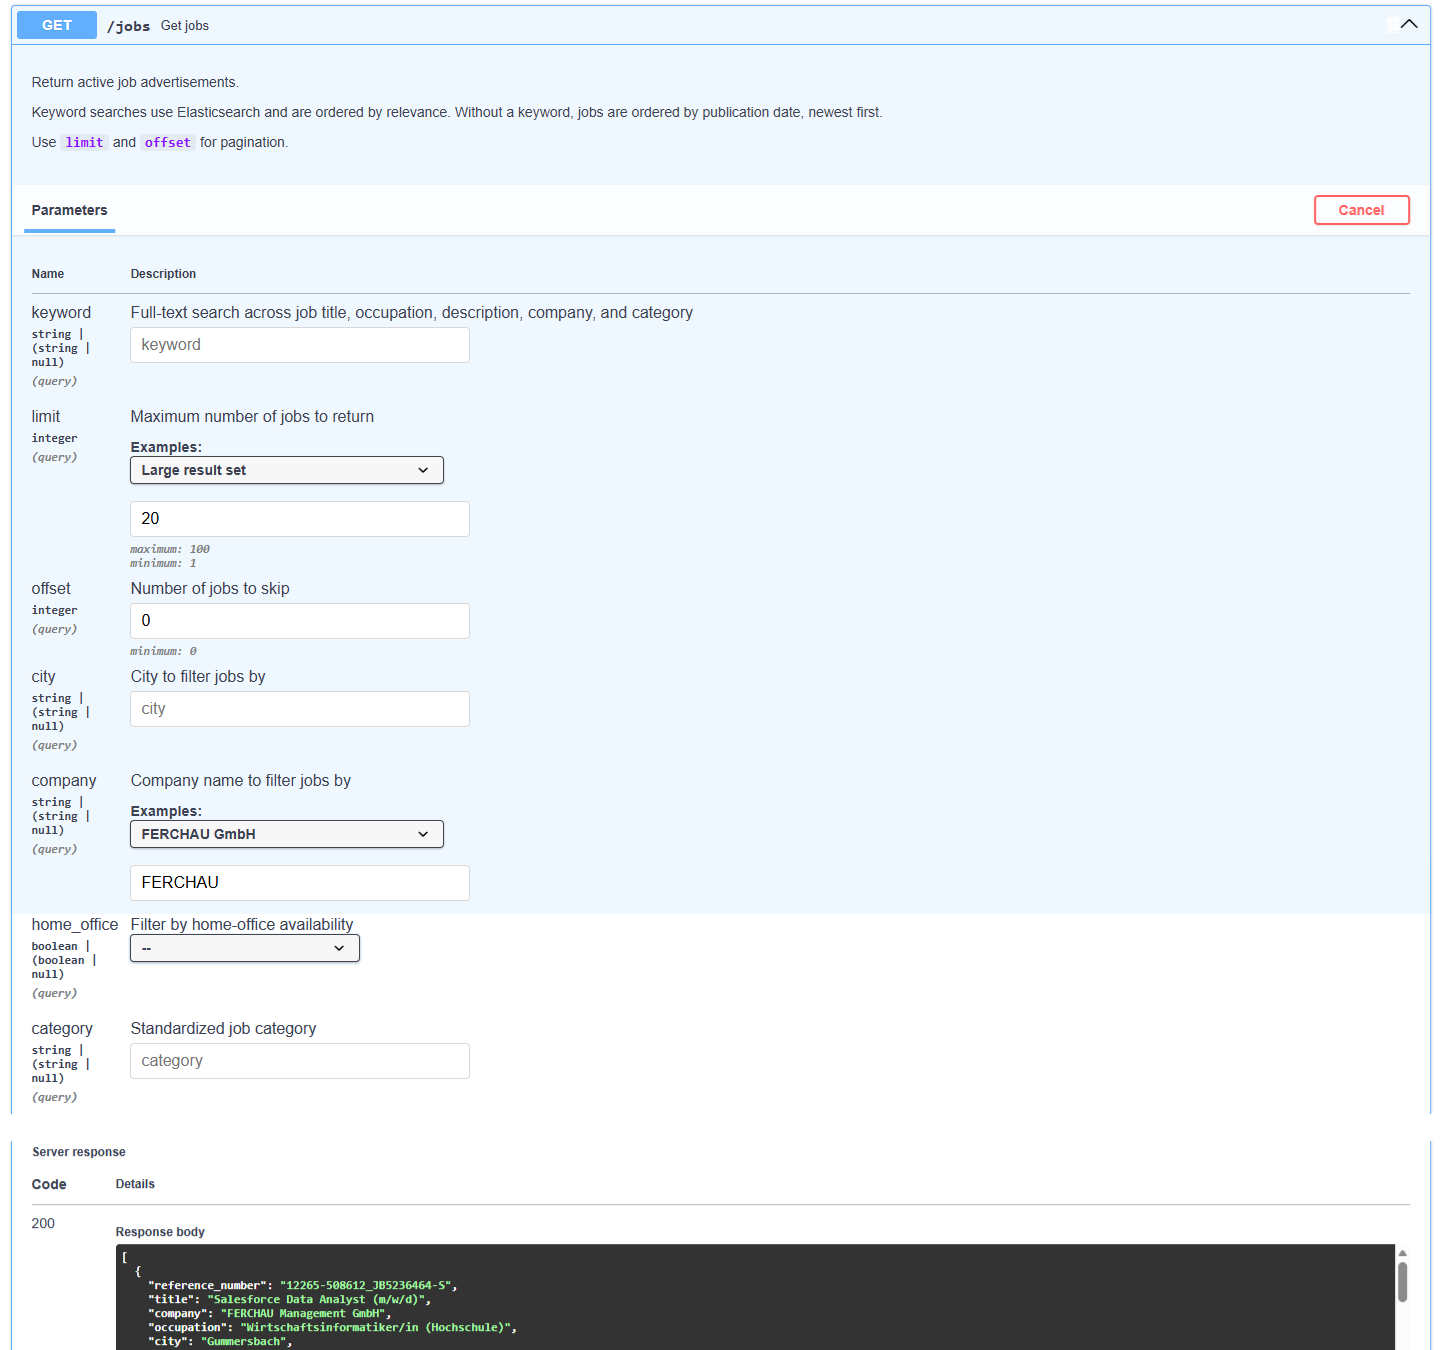
\includegraphics[width=\textwidth]{swagger-jobs.png}
	\caption{Swagger interface for the \texttt{GET /jobs} endpoint with search, filter, and pagination parameters.}
	\label{fig:swagger-jobs}
\end{figure}

The detail endpoint \path{/jobs/{reference_number}} uses the source reference number to retrieve the complete advertisement and all related locations. Unlike the  \path{/jobs} endpoint, it can also return advertisements that are no longer active. An unknown reference number produces HTTP~404.

Figure~\ref{fig:swagger-job} illustrates a successful detail request and the returned HTTP~200 response.

\begin{figure}[htbp]
	\centering
	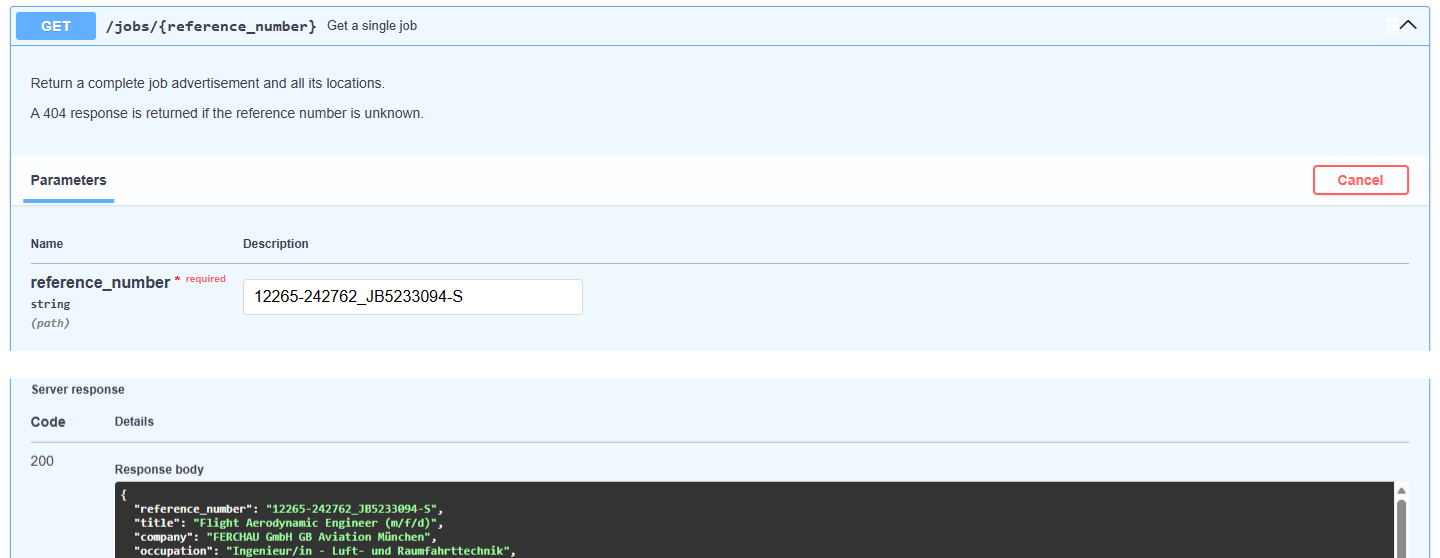
\includegraphics[width=\textwidth]{swagger-job.png}
	\caption{Swagger interface for the \texttt{GET /jobs/\{reference\_number\}} endpoint and a successful detail response.}
	\label{fig:swagger-job}
\end{figure}

Although an advertisement may contain several locations, the \path{/jobs} endpoint returns only one location for each job. When a city filter is supplied, a location matching that city is selected, favouring one with coordinates where available. If no city filter is supplied, a location with available coordinates is selected where possible. The detail endpoint always returns the complete location list.

This API is also consumed by the frontend, keeping filtering, pagination, search, and database access in the backend while the dashboard remains responsible for presentation.

\subsection{Full-Text Search and Structured Filtering}

The job-search endpoint distinguishes between free-text search and field-based filtering. The API parameter \path{keyword} contains the user's free-text search query and triggers a relevance-oriented Elasticsearch search, while parameters such as \path{city}, \path{company}, \path{home_office}, and \path{category} restrict the eligible result set. This parameter is unrelated to both the search terms used with the Bundesagentur für Arbeit API during data collection and Elasticsearch's \path{keyword} field type.

Figure~\ref{fig:elasticsearch-search} presents the search process from two perspectives. The left side shows how requests are routed depending on whether a free-text keyword is supplied, while the right side shows the interaction between FastAPI, Elasticsearch, and PostgreSQL during a keyword search.

\begin{figure}[htbp]
	\centering
	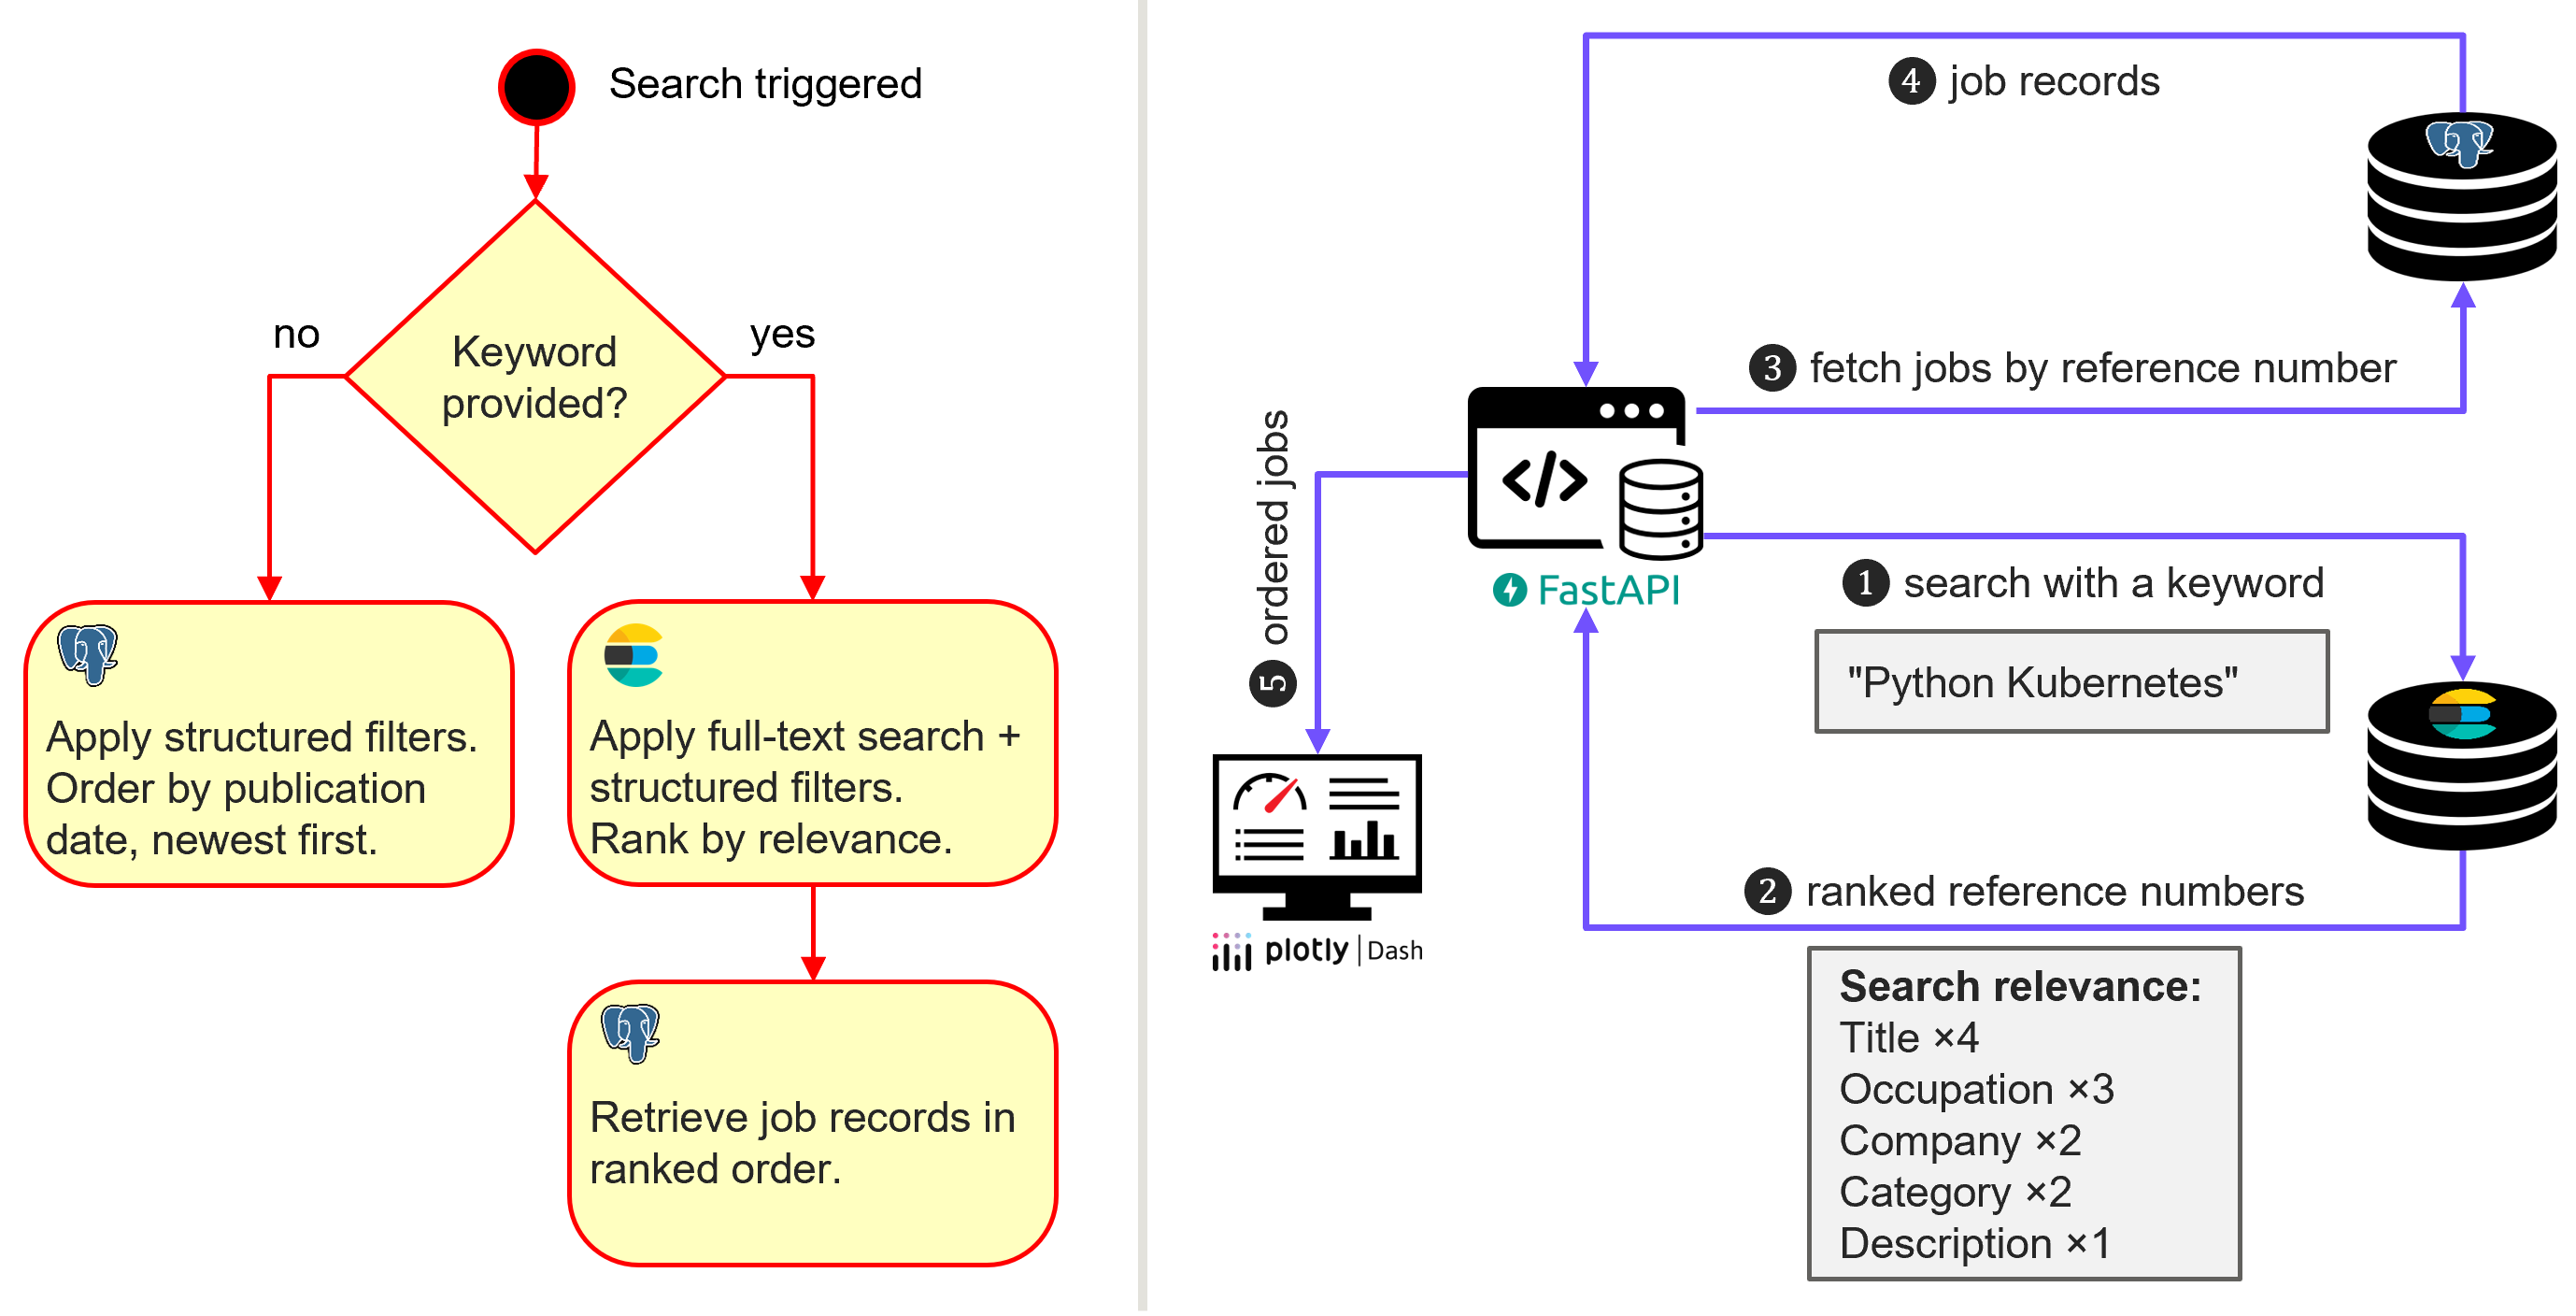
\includegraphics[
	width=\textwidth,
	keepaspectratio
	]{elasticsearch.png}
	\caption{Job-search processing. The left side shows the routing between PostgreSQL-based filtering and Elasticsearch-based full-text search; the right side shows the Elasticsearch search path, relevance ranking, and subsequent retrieval of job records from PostgreSQL.}
	\label{fig:elasticsearch-search}
\end{figure}

As shown on the left side of Figure~\ref{fig:elasticsearch-search}, requests without a keyword are handled entirely by PostgreSQL. The field-based filters are applied directly to the database, and the matching jobs are ordered by publication date. When a keyword is supplied, the filters are instead included in the Elasticsearch query together with the full-text search. Elasticsearch returns the matching reference numbers in relevance order, after which the corresponding job records are retrieved from PostgreSQL while preserving that order.

The right side of Figure~\ref{fig:elasticsearch-search} shows this keyword-search path in more detail. Keyword searches use an Elasticsearch \path{multi_match} query across title, occupation, company, category, and description. The fields are weighted heuristically according to how directly they are expected to represent the user's search intent: the title receives the highest boost because it most directly identifies the advertised role, followed by occupation, whereas company and category provide broader or more indirect signals, and the description receives the lowest weight because it contains substantially more text and may include many incidental terms. As a result, matches in more heavily weighted fields contribute more strongly to the ranking. The corresponding relevance weights are also listed on the right side of the figure.

As discussed in Section~\ref{subsec:elasticsearch-index-sync}, PostgreSQL remains the authoritative source of job data, while Elasticsearch provides specialised full-text search, filtering, and relevance ranking.


\subsection{Statistics API}

In addition to individual job retrieval, the FastAPI backend exposes read-only statistical endpoints under the \path{/statistics} prefix. These endpoints perform SQL aggregations directly on PostgreSQL and provide the data consumed by the Statistics page of the Dash frontend.

The available statistics include an overview of the dataset, the most frequently occurring companies and locations, home-office availability, job-category distribution, and monthly publication trends. Location statistics are based on distinct job advertisements rather than on the number of stored location rows. Since one advertisement may be associated with several locations, counting the rows directly could count the same job more than once. Home-office availability distinguishes between \path{possible}, \path{not_possible}, and \path{unknown}, preventing missing source information from being interpreted as a negative value.

The publication-trends endpoint groups advertisements by the month of their \path{first_publication_date} and returns the resulting counts in chronological order. Figure~\ref{fig:swagger-trends} shows an example of this monthly aggregation.

\begin{figure}[htbp]
	\centering
	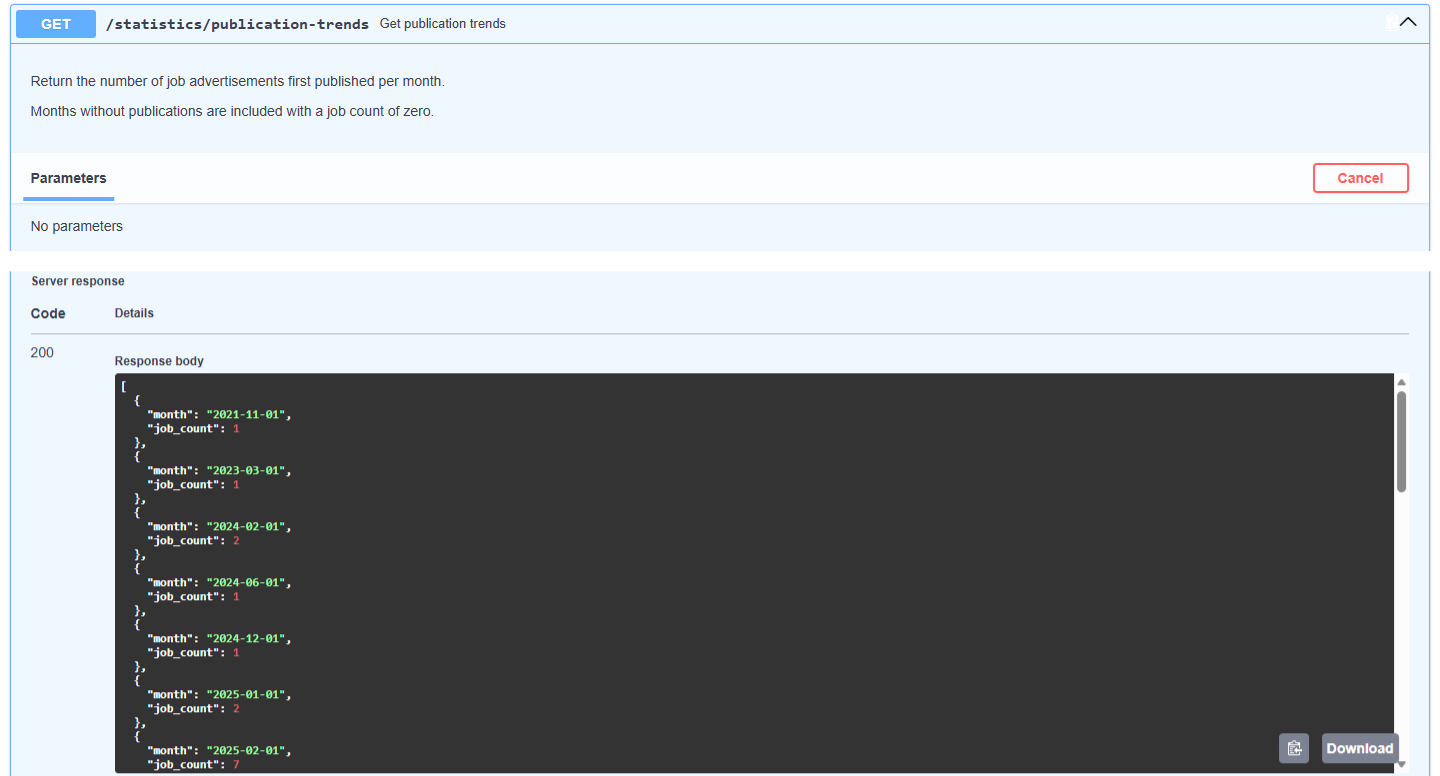
\includegraphics[width=0.95\textwidth]{swagger-trends.png}
	\caption{Swagger interface for the \texttt{GET /statistics/publication-trends} endpoint showing monthly publication counts.}
	\label{fig:swagger-trends}
\end{figure}


\subsection{Dash Frontend}

The Dash application provides the user-facing interface for exploring the collected job advertisements. It communicates exclusively with the FastAPI backend and does not access PostgreSQL directly. The main \textit{Find jobs} view combines search controls, a paginated result list, and an interactive map, as shown in Figure~\ref{fig:job-search-interface}.

\begin{figure}[!ht]
	\centering
	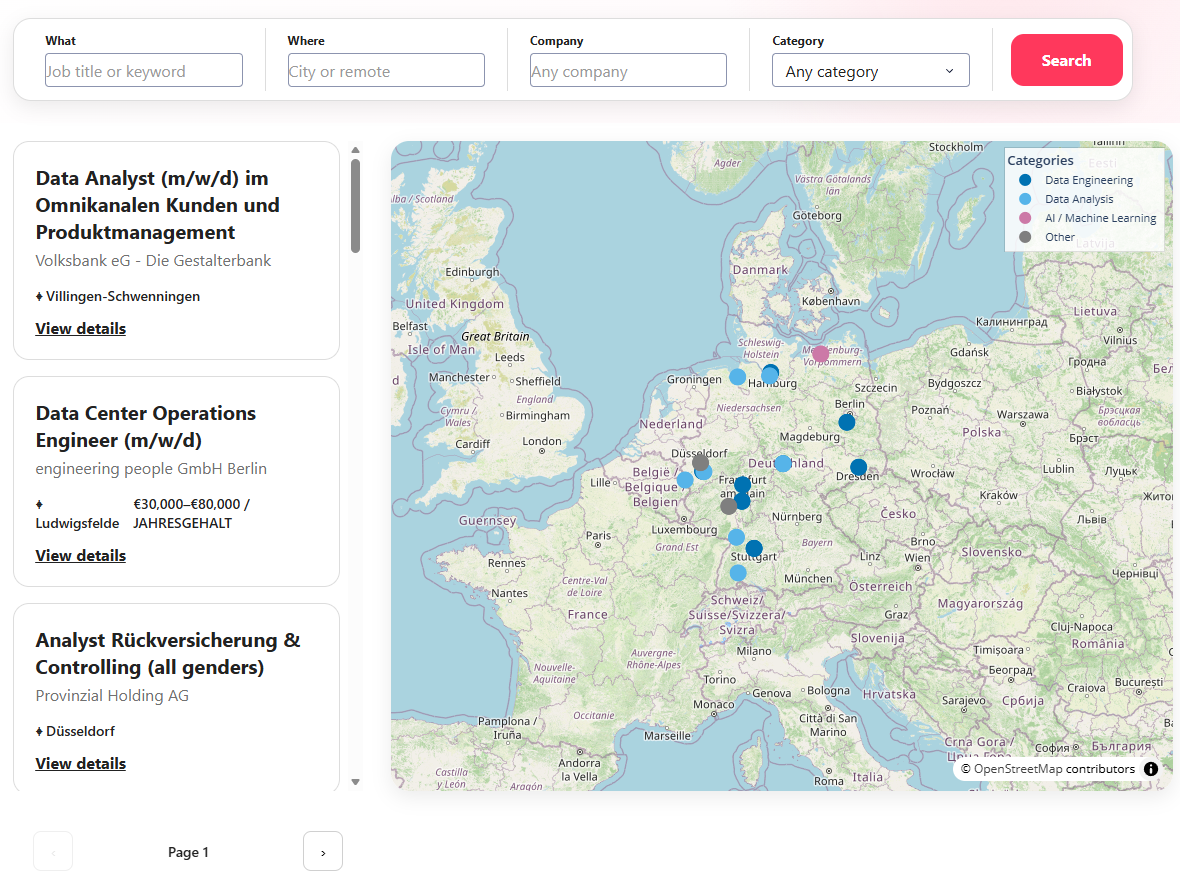
\includegraphics[
	width=\textwidth,
	height=0.75\textheight,
	keepaspectratio
	]{find-jobs-ui.png}
	\caption{Job search interface with filters, results, and an interactive map.}
	\label{fig:job-search-interface}
\end{figure}

The search controls correspond to the main filters exposed by the \path{/jobs} endpoint. Results are displayed as paginated cards and, where geographic coordinates are available, as category-coloured markers on the map. The list and map are therefore complementary representations of the same API response rather than independent data sources.

Detailed information is loaded only when requested. Selecting a result card or map marker triggers a request to \path{/jobs/{reference_number}} and opens a modal containing the complete advertisement, including its locations, description, publication and freshness information, and an external link when available.

The \textit{Statistics} view presents aggregated information retrieved from the Statistics API, including overview of the dataset, publication trends, leading companies and locations, home-office availability, and job-category distribution. The frontend also distinguishes technical backend failures from valid empty results by displaying an explicit error message when API requests cannot be completed.


\subsection{Visual Analytics}

The Statistics view complements the search-oriented interface by aggregating the collected advertisements into broader indicators of employer activity, geographical concentration, home-office availability, job-category distribution, and publication trends. Figure~\ref{fig:statistics-interface} shows the location, home-office, and category views provided by the Dash Statistics page.

\begin{figure}[!ht]
	\centering
	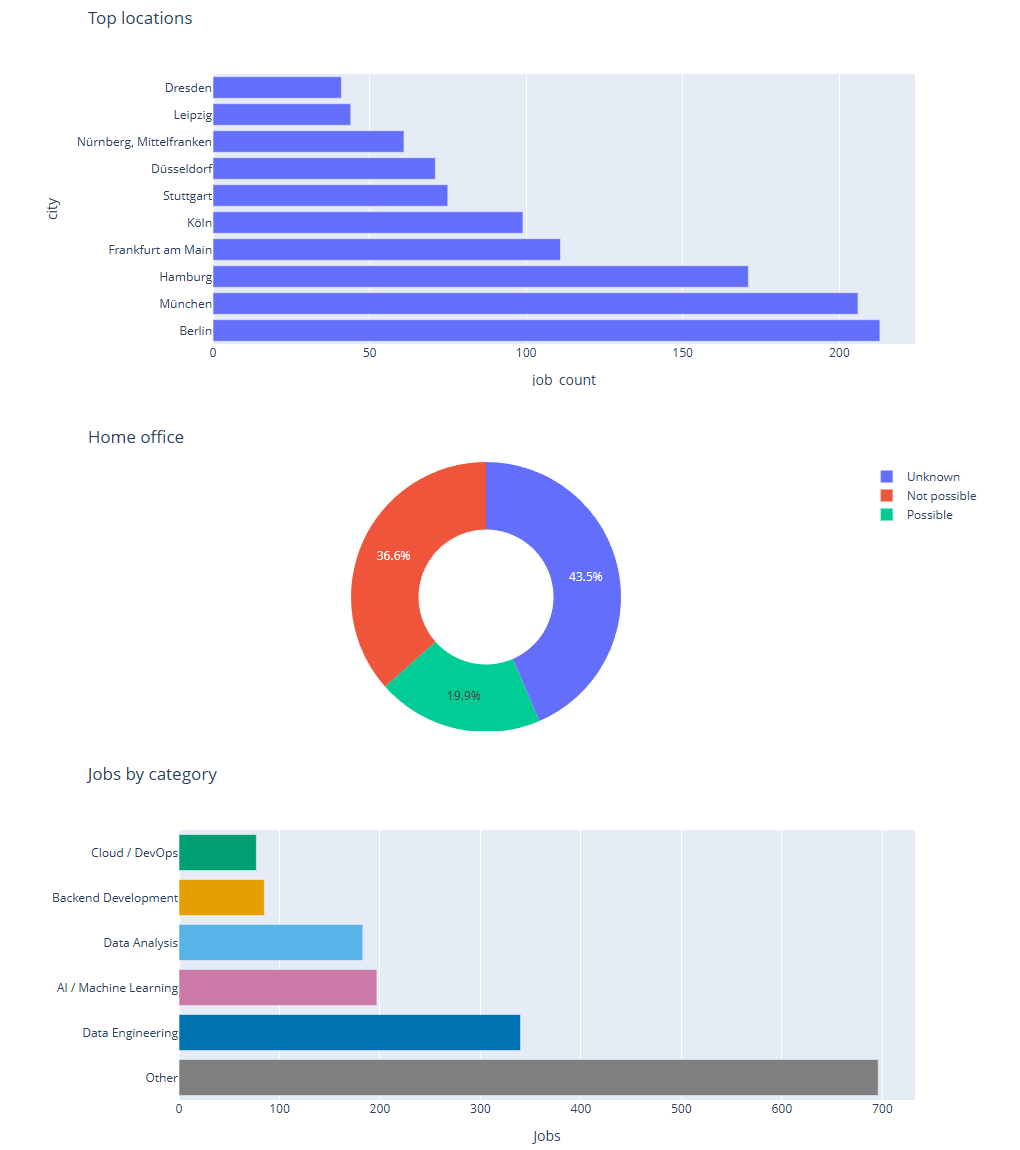
\includegraphics[width=\textwidth]{statistics-ui.png}
	\caption{Dash visual analytics showing leading job locations, reported home-office availability, and the distribution of standardised job categories.}
	\label{fig:statistics-interface}
\end{figure}

The company and location rankings show which employers and cities are most strongly represented in the collected dataset. These values should not be interpreted as complete rankings of the German labour market, since they depend on the selected data source and configured search terms.

The home-office distribution distinguishes between advertisements that explicitly report home office as possible, not possible, or provide no corresponding information. Treating missing values as \textit{Unknown} avoids interpreting absent source information as a negative answer and also reveals the incompleteness of this attribute.

The category distribution provides a higher-level view of the technical job profiles represented in the dataset. Because job titles and occupation labels are mapped to the standardised categories described in Section~\ref{sec:job-classification}, advertisements with different wording can be grouped into the same category.

The Statistics page additionally provides a time-series view based on each advertisement's first publication month. It supports exploratory analysis over different time ranges.




\section{Deployment and Automation}


\subsection{Docker Compose Deployment}

The complete application is containerised with Docker and orchestrated through Docker Compose. Figure~\ref{fig:docker-deployment} shows the principal services and their communication paths.

\begin{figure}[!ht]
	\centering
	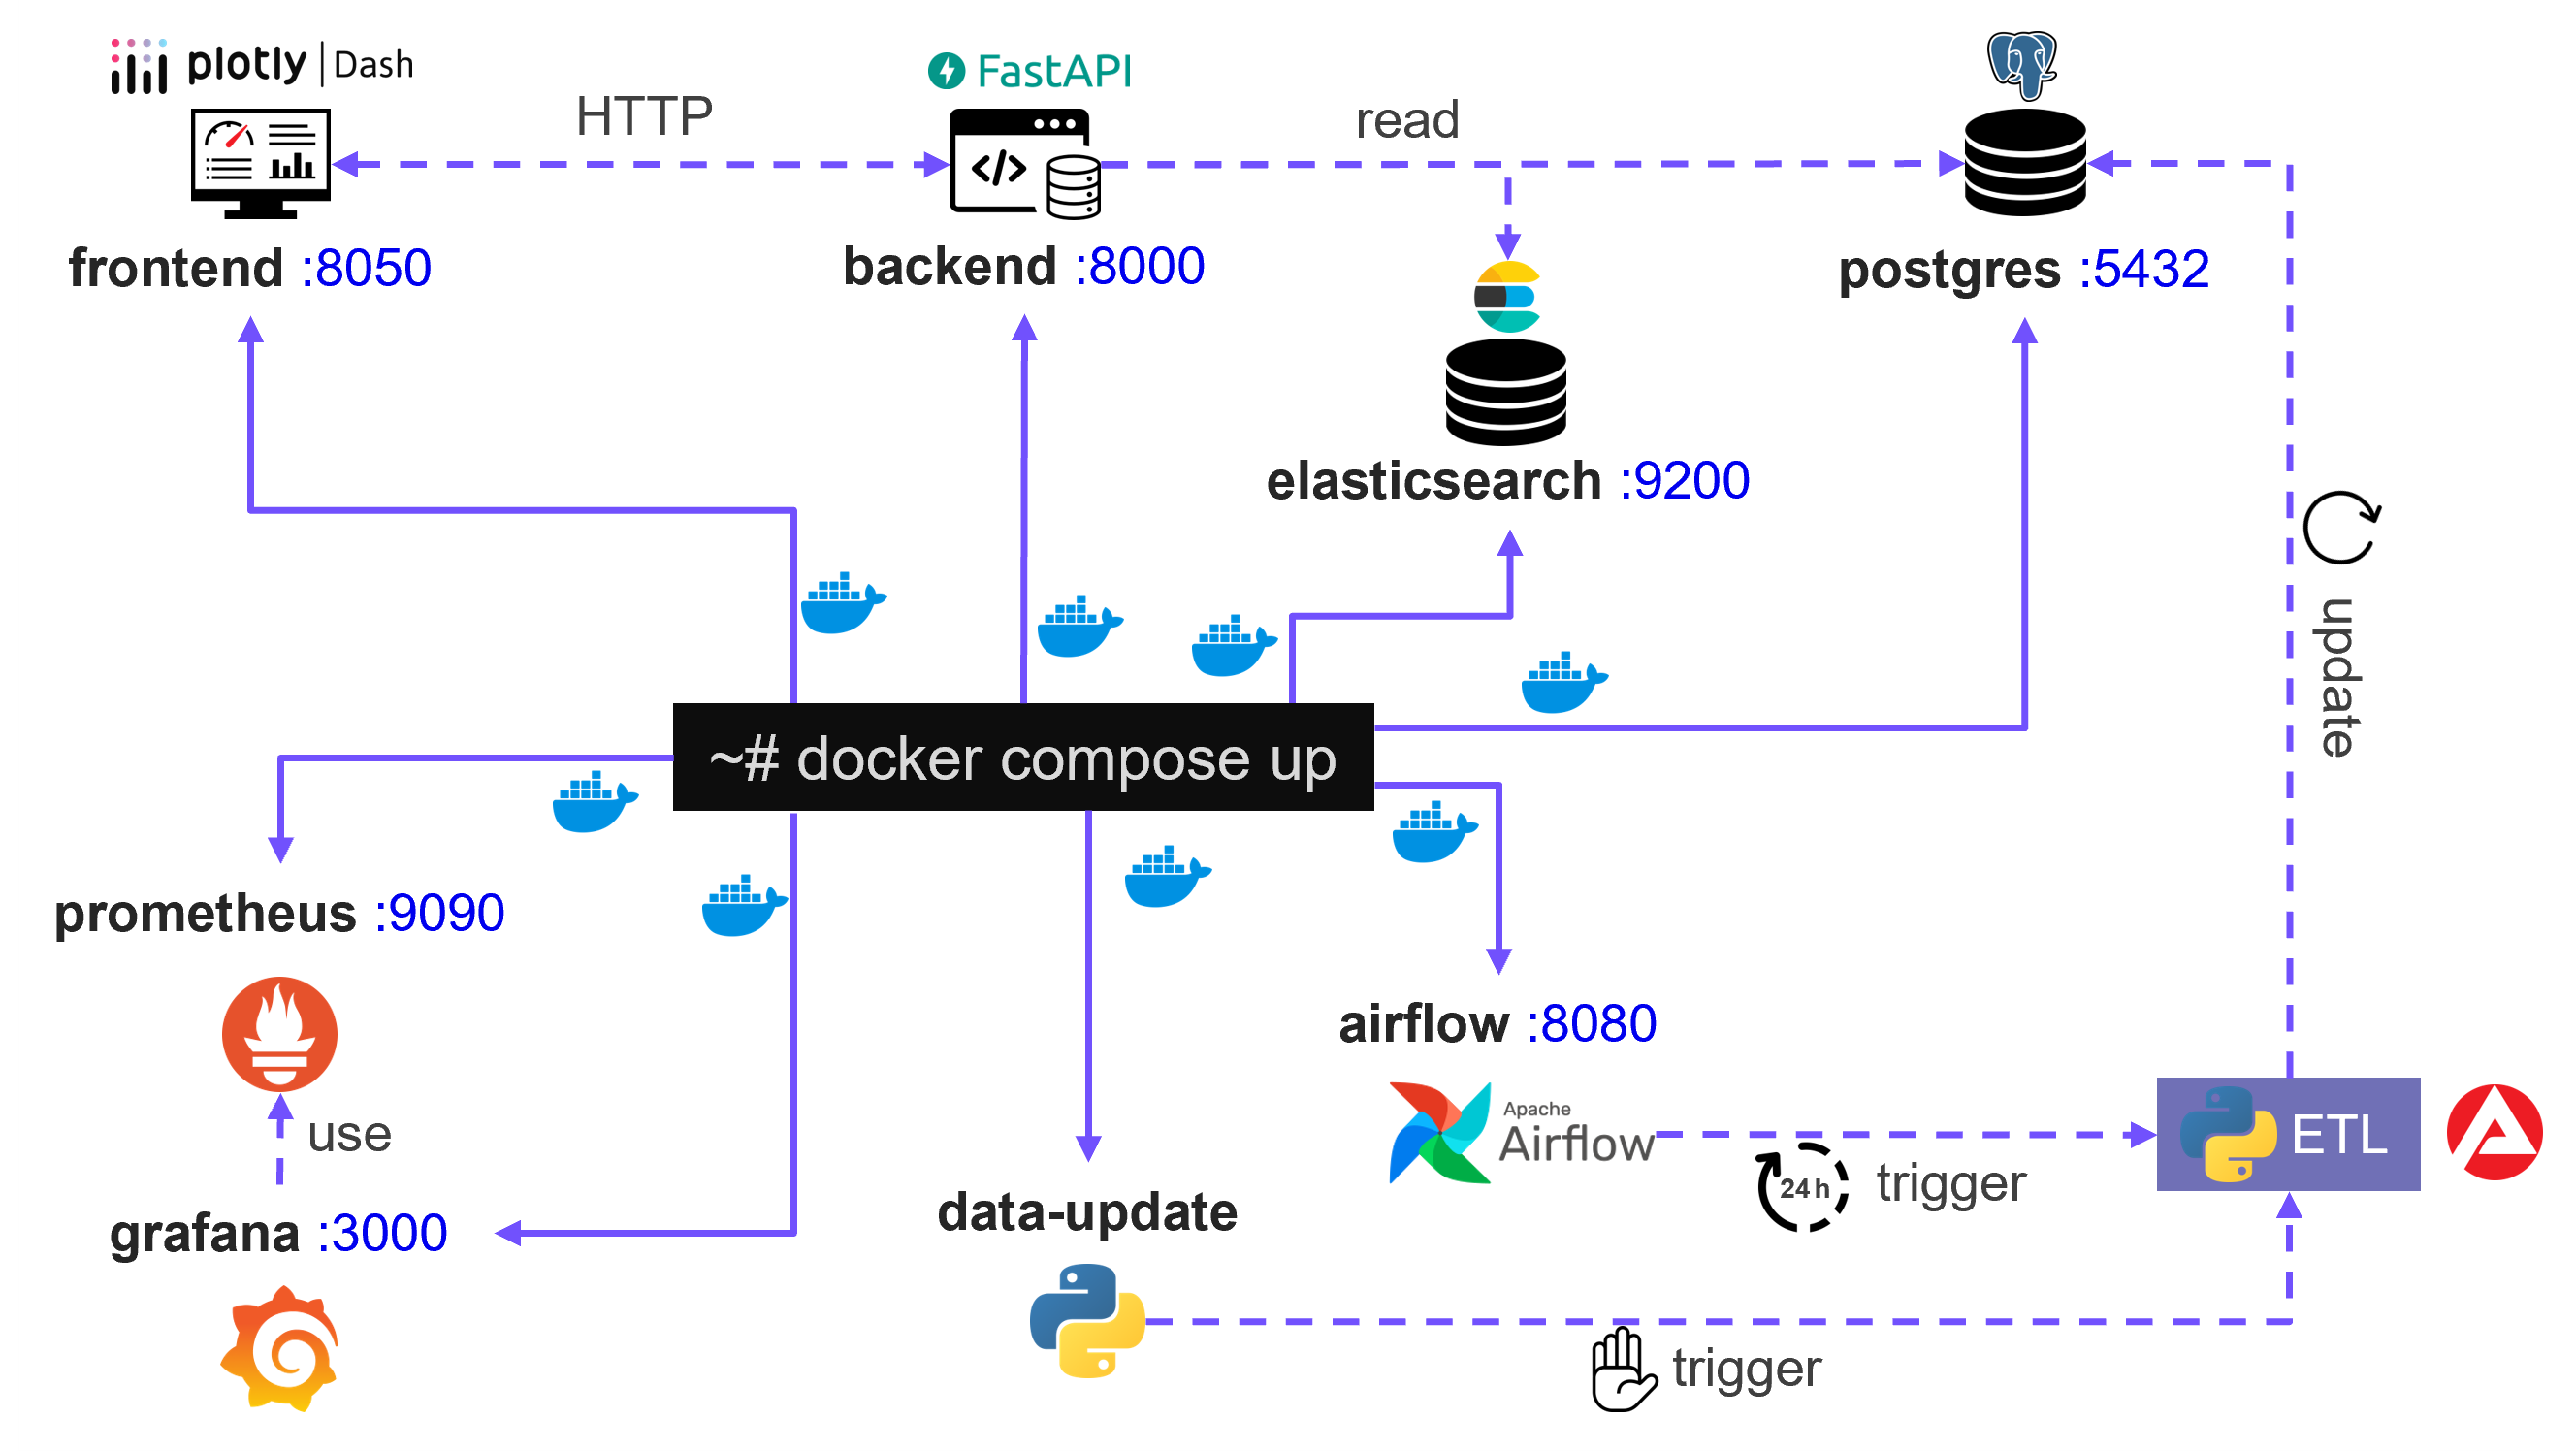
\includegraphics[
	width=\textwidth,
	height=0.75\textheight,
	keepaspectratio
	]{docker-deployment.png}
	\caption{Containerised deployment and communication between services.}
	\label{fig:docker-deployment}
\end{figure}

The FastAPI backend, Dash frontend, and manual \path{data-update} service use the same Python application image but execute different commands at runtime. This avoids maintaining several nearly identical images and ensures that these components use the same application code and dependencies. Airflow uses a separate image based on the official Airflow distribution because it requires its own runtime and directory structure, while infrastructure components such as PostgreSQL, Prometheus, Pushgateway, Alertmanager, Grafana, and Elasticsearch use their respective standard images.

Docker Compose connects the services through an internal network. FastAPI accesses PostgreSQL and Elasticsearch through their service names, while Dash communicates only with FastAPI and does not access the data stores directly. Service dependencies and health checks ensure that components such as the backend and ETL do not start before their required data services are available.

Data ingestion can be executed through two paths. The \path{data-update} service provides an on-demand ETL environment, while Airflow executes the pipeline automatically according to its configured schedule. Both use the same ETL implementation and access the shared persistent data required by the pipeline.

Persistent state is stored in Docker volumes rather than inside the container filesystems, allowing PostgreSQL data, Elasticsearch data, archived ETL files, Prometheus time series, and Grafana state to survive container recreation. Monitoring configuration, alert rules, and dashboard definitions are stored as files in the project repository and mounted into the corresponding containers, separating persistent runtime state from reproducible configuration.


\subsection{ETL Orchestration with Airflow}

Apache Airflow orchestrates the recurring ingestion pipeline by scheduling and sequencing the existing extraction, transformation, loading, freshness-tracking, and Elasticsearch synchronisation functions. The Airflow tasks act as thin wrappers around these functions, keeping orchestration separate from the ETL implementation. The DAG follows this dependency chain:

\[
\begin{array}{rcl}
	\texttt{start monitoring}
	& \rightarrow & \texttt{extract} \rightarrow \texttt{transform} \rightarrow \texttt{load} \\
	& \rightarrow & \texttt{update freshness} \rightarrow \texttt{update elasticsearch} \\
	& \rightarrow & \texttt{publish metrics}
\end{array}
\]

The monitoring-specific first and final tasks are described in Section~\ref{sec:collected-metrics}. Extraction produces the raw-data directory and the set of job reference numbers observed during the current search. The transformed data is subsequently loaded into PostgreSQL before freshness information is updated, as described in Section~\ref{sec:loading}, ensuring that advertisement state is not changed before the current dataset has been processed successfully. Finally, the Elasticsearch index is synchronised with the updated set of active jobs, as discussed in Section~\ref{subsec:elasticsearch-index-sync}.

The DAG is scheduled with the cron expression \texttt{0 6 * * *}, resulting in one automated run every day at 06:00. The configuration \path{catchup=False} ensures that Airflow does not try to execute all previously missed daily runs when the DAG is started or re-enabled.




\section{Monitoring and Reliability}


\subsection{Monitoring Architecture}

The project monitors both the continuously running FastAPI backend and the periodically executed ETL pipeline. As shown in Figure~\ref{fig:monitoring-architecture}, backend metrics can be scraped directly by Prometheus, whereas the short-lived ETL process publishes its latest metrics through Pushgateway.

\begin{figure}[htbp]
	\centering
	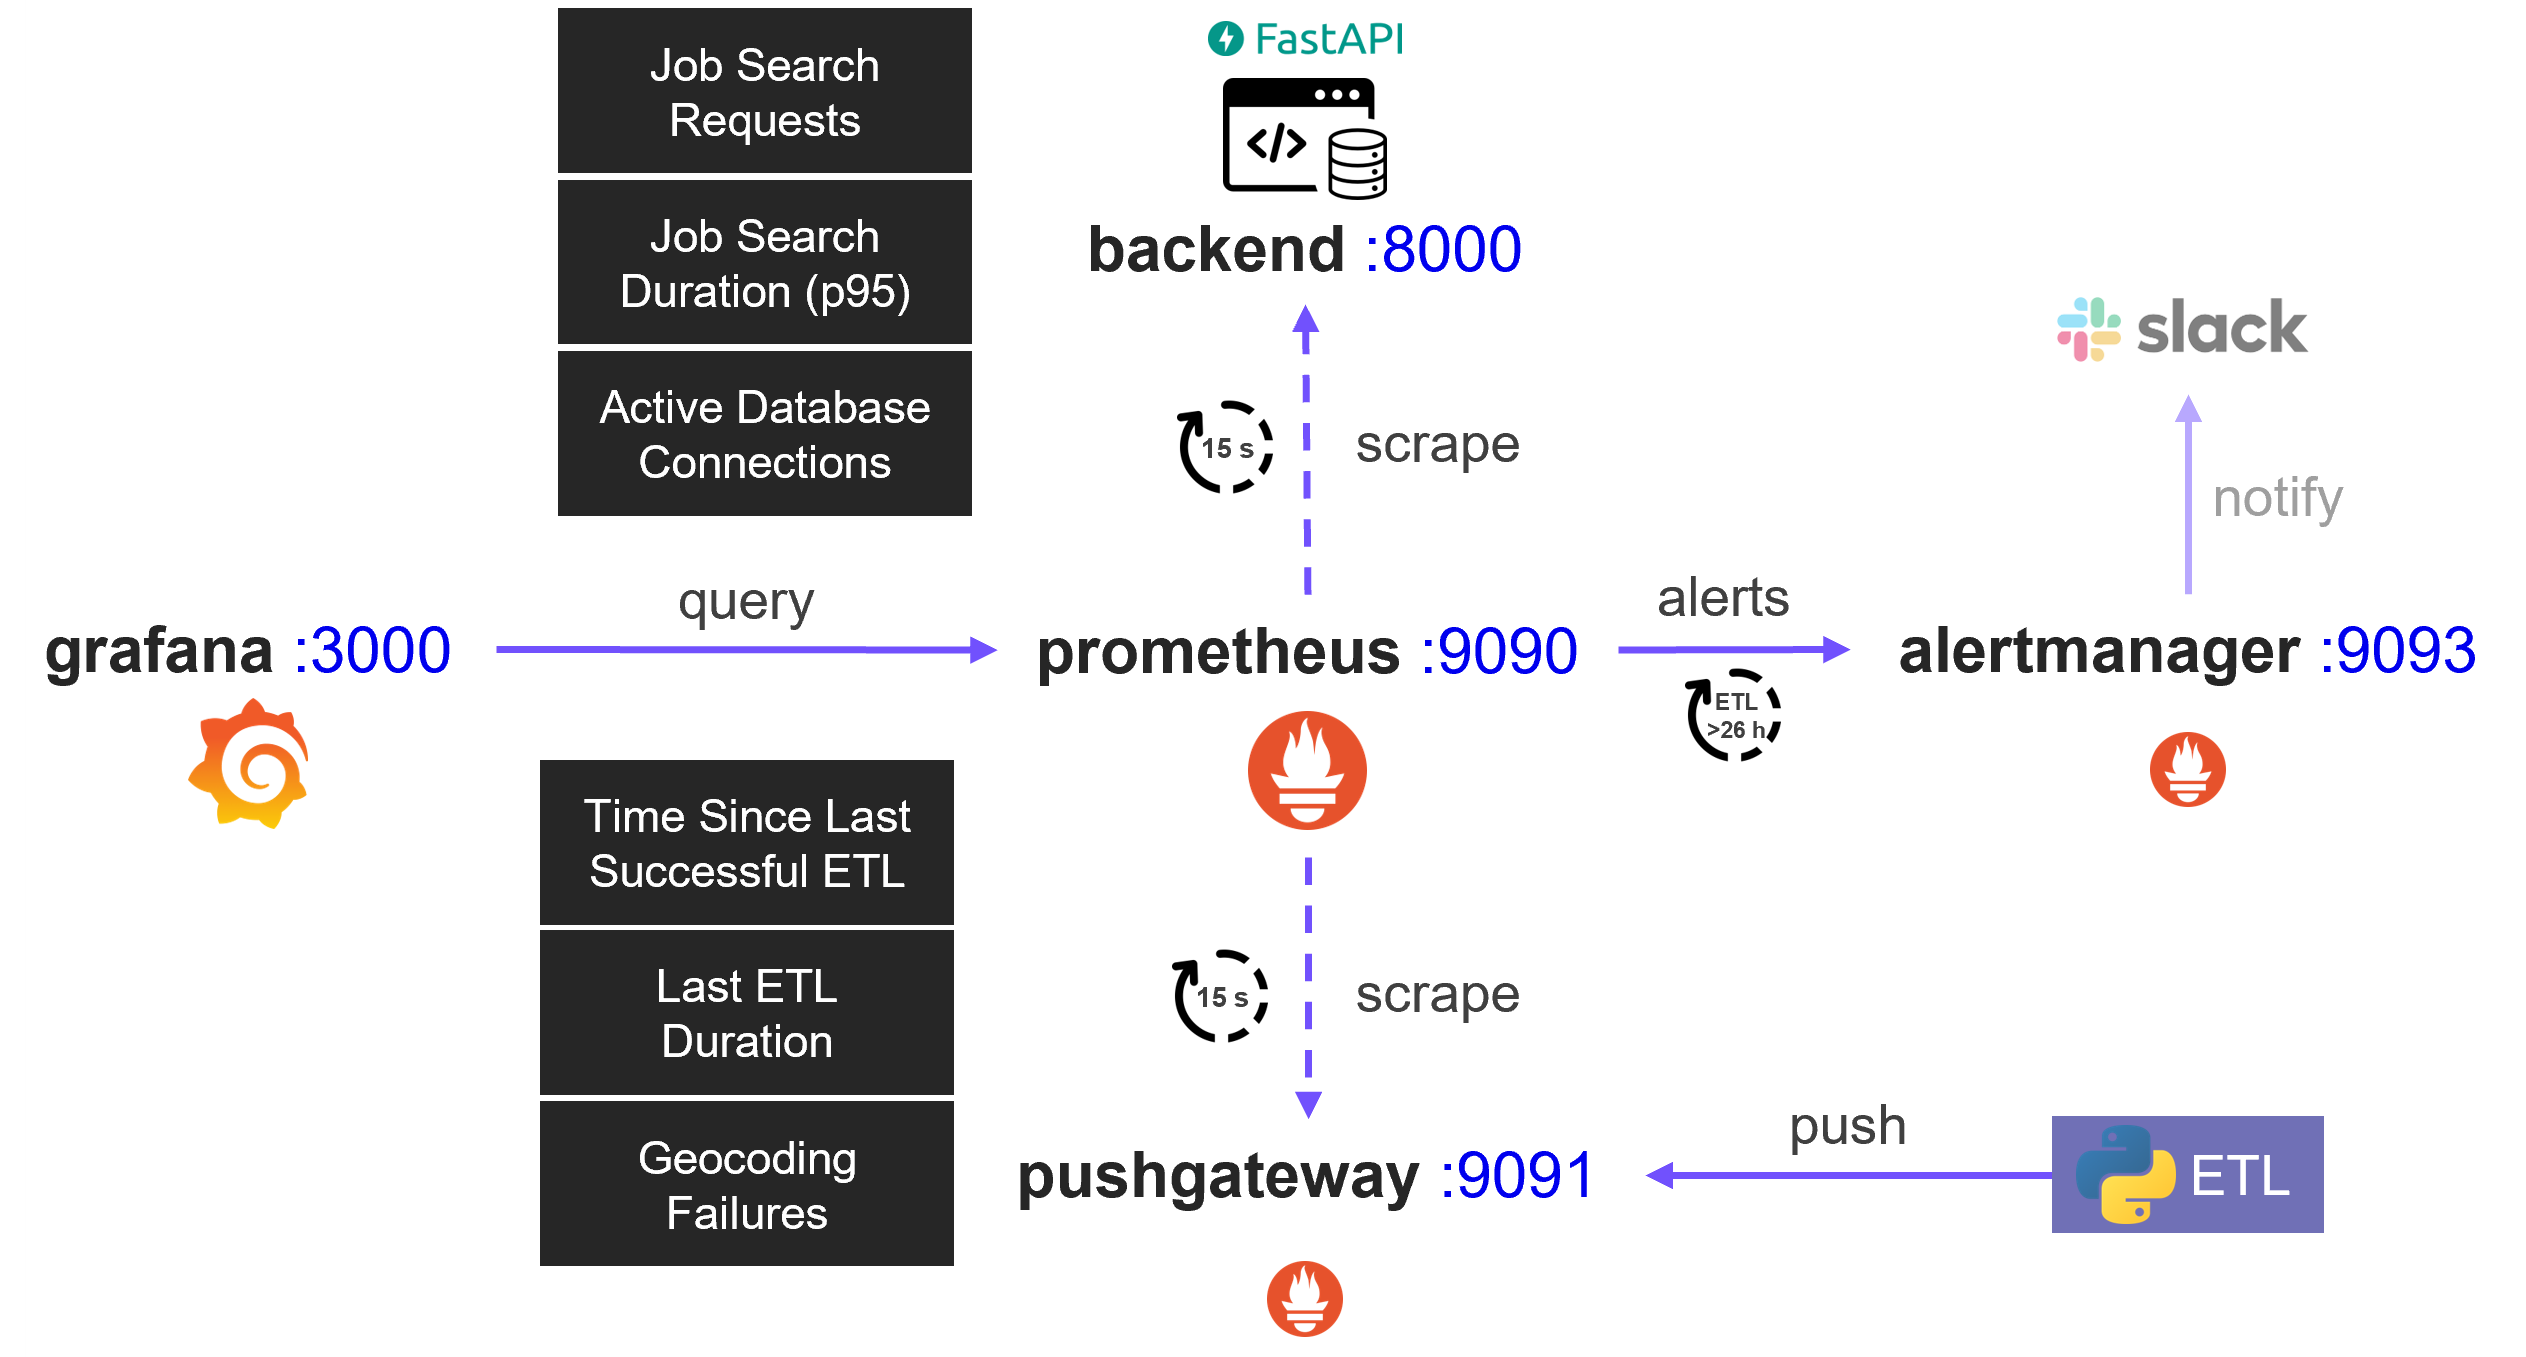
\includegraphics[
	width=\textwidth,
	height=0.75\textheight,
	keepaspectratio
	]{monitoring.png}
	\caption{Monitoring architecture using Prometheus, Pushgateway, Grafana, and Alertmanager. Slack represents an optional notification integration.}
	\label{fig:monitoring-architecture}
\end{figure}

The backend exposes Prometheus metrics for job-search activity and duration, database connections, and requests to the Bundesagentur für Arbeit API. ETL metrics include the duration and timestamp of the latest successful run as well as failed geocoding requests. Prometheus collects metrics from both monitoring paths and makes them available for querying and visualisation.

Grafana uses Prometheus as its datasource and visualises metrics from both monitoring paths, including request activity and latency, active database connections, ETL duration and freshness, and geocoding failures. Prometheus therefore provides metric collection and storage, while Grafana provides the visual monitoring layer.

Prometheus also evaluates an alert for overdue ETL execution. The alert is triggered when the last successful run is more than 26 hours old for at least 30 minutes, allowing two hours of tolerance beyond the daily schedule. Alerts are forwarded to Alertmanager for routing. No external notification channel is currently configured, although services such as Slack could be integrated with minimal additional configuration as a production extension.


\subsection{Collected Metrics \label{sec:collected-metrics}}

The monitoring instrumentation covers both external dependencies and local application activity, including the Bundesagentur für Arbeit API, PostgreSQL access, job-search requests, and ETL execution. Requests to the Bundesagentur für Arbeit are monitored through request counts by operation and outcome and through request-duration histograms, while a separate gauge records whether the most recent request succeeded. PostgreSQL access in the backend is monitored by tracking the number of database connections concurrently in use.

Job-search requests are monitored through request counts and request-duration histograms. Grafana uses these metrics to display search activity and the 95th-percentile response duration, providing visibility into both request volume and API responsiveness.

ETL monitoring records the duration and timestamp of the latest successful run. The \path{failed_geocoding_requests} metric is reset before geocoding begins and incremented whenever a geocoding lookup fails, recording the number of unsuccessful lookups during that run.

Figure~\ref{fig:grafana-dashboard} shows the Grafana dashboard used to inspect selected application and ETL metrics.

\begin{figure}[htbp]
	\centering
	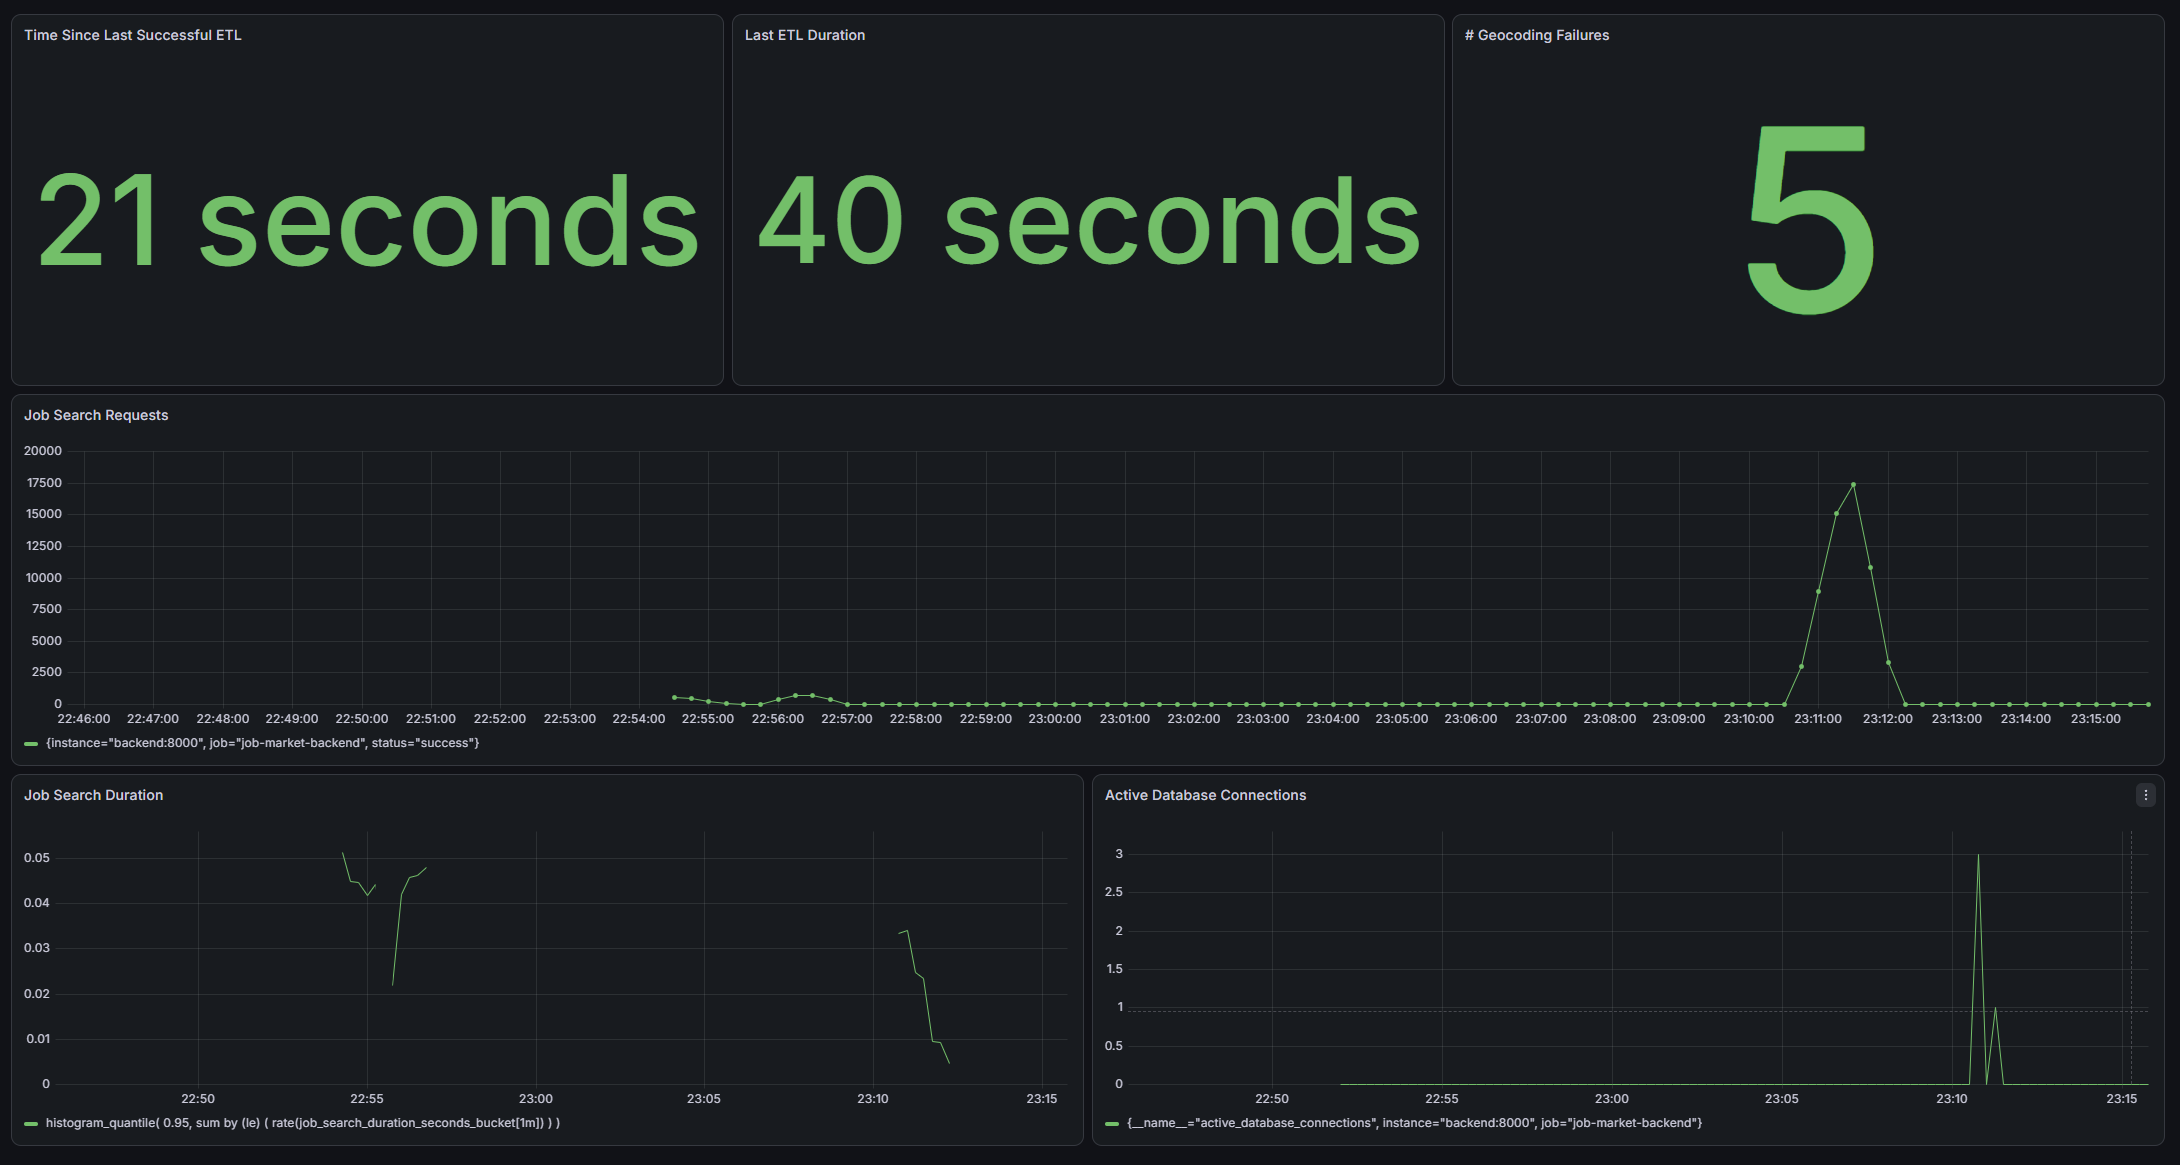
\includegraphics[
	width=\textwidth,
	height=0.58\textheight,
	keepaspectratio
	]{grafana-screenshot.png}
	\caption{Grafana dashboard displaying ETL freshness and duration, geocoding failures, job-search activity and duration, and active database connections.}
	\label{fig:grafana-dashboard}
\end{figure}

The dashboard combines ETL freshness and duration with job-search activity and response duration, geocoding failures, and concurrent database usage. In the local test run shown in Figure~\ref{fig:grafana-dashboard}, the increase in job-search requests coincides with an increase in the number of database connections in use, illustrating how related metrics can be inspected together. The values were generated for demonstration purposes and should not be interpreted as a general performance benchmark.


\subsection{Error Handling}

Error handling is designed to isolate failures where possible rather than terminate the complete pipeline or application. Failed source requests and malformed records are logged and skipped while unaffected advertisements continue to be processed. In particular, unsuccessful job-detail requests are recorded separately, and temporary failures during freshness checks do not cause previously active advertisements to be marked inactive.

Infrastructure failures are exposed explicitly to application clients. If PostgreSQL is unavailable, the relevant FastAPI endpoints return HTTP~503, whereas requests for unknown job references return HTTP~404. This distinction allows clients to differentiate service failures from valid requests that simply return no matching data.

Failures of optional enrichment services are also non-fatal: unsuccessful geocoding leaves locations without coordinates and is recorded through monitoring metrics. ETL success metrics are updated only after a successful pipeline run, so failed executions remain visible through the unchanged last-success timestamp and can trigger the corresponding Prometheus alert.


%	\subsection{Automated Tests and Continuous Integration}
%	category-classification tests;
%	short-keyword boundary test;
%	classification-priority test;
%	smoke test;
%	GitHub Actions checks: Black, pytest, and Docker image build.




\section{Results and Evaluation}


\subsection{Achieved Results}

The project delivers a functional end-to-end data-engineering system for collecting, processing, storing, and exploring German job advertisements. The pipeline retrieves advertisements from the Bundesagentur für Arbeit, preserves timestamped raw data, transforms and enriches the source records, and loads them into PostgreSQL. Repeated runs update existing advertisements without duplication while preserving freshness information and distinguishing genuine modifications from unchanged republications.

The processed data is exposed through FastAPI and consumed by a Dash frontend that supports job search, field-based filtering, full-text search, geographic exploration, job details, and aggregated statistics. Elasticsearch extends the application with relevance-based full-text search, while PostgreSQL provides the stored job records used by the API.

The complete workflow can be executed automatically through Airflow and runs in a reproducible Docker Compose environment. Monitoring is provided for both the application and the periodic ETL process. Overall, the project integrates data acquisition, historisation, relational storage, search, API-based access, visual analytics, workflow orchestration, containerised deployment, and operational monitoring into a coherent data platform.


\subsection{Technical Decisions}

The storage design deliberately separates source preservation from operational data access. Timestamped JSON files retain the original API responses for traceability and reprocessing, while PostgreSQL stores the transformed relational representation used by the application. PostgreSQL was preferred over querying JSON files or introducing a document database because the stable job and location model benefits directly from relational constraints, transactions, joins, indexing, and conflict-aware updates.

The application separates data access from presentation through FastAPI. Dash communicates exclusively with the API rather than with PostgreSQL, keeping filtering, validation, statistics, and persistence logic in the backend. Dash was chosen because the project emphasises data engineering and analytical visualisation and therefore benefits from a Python-based frontend without the additional complexity of a separate JavaScript application.

Elasticsearch complements rather than replaces PostgreSQL. It is used for full-text search and relevance ranking, while PostgreSQL remains the authoritative data store for persisted job data and record retrieval. The Elasticsearch index is therefore treated as a rebuildable projection of the active database state, avoiding the consistency problems of maintaining two independent sources of truth.

Docker Compose was chosen to provide a reproducible multi-service environment without introducing the operational complexity of a distributed deployment platform. Airflow was added to express the dependencies and schedule of the recurring ETL workflow explicitly. The monitoring stack was designed to cover both continuously running services and the short-lived ETL process, providing observability appropriate to the project scope without requiring production-scale infrastructure.


\subsection{Limitations}

The collected dataset does not represent the complete German labour market. The project uses the Bundesagentur für Arbeit as its only data source and regularly collects advertisements only for the configured search keywords. Jobs published exclusively elsewhere are therefore absent, and frequently missing attributes such as salary, home-office availability, or location information further limit some analyses. Statistical results should consequently be interpreted as characteristics of the collected sample rather than as exhaustive labour-market statistics.

Temporal analysis is also limited by the observation period. Source publication dates do not constitute a complete historical census, while project-generated freshness information accumulates only after the pipeline begins observing an advertisement. Reliable conclusions about long-term changes in the job market therefore require continuous operation over a longer period.

Job classification relies on deterministic keyword rules applied to titles and occupations. Although transparent and reproducible, this approach cannot fully capture semantic context, uncommon terminology, or jobs spanning several disciplines. The resulting categories are therefore suitable for filtering and exploratory analysis but not as an authoritative occupational taxonomy.

Elasticsearch is deployed as a single-node search index and is rebuilt after each scheduled ingestion. This approach is sufficient for the current dataset but would become inefficient at larger scale and can temporarily affect full-text search during synchronisation. Incremental indexing or atomic index replacement would be preferable in a production system.

Location enrichment depends partly on the external Nominatim service. Geocoding can fail for incomplete or ambiguous locations or during service interruptions, leaving some jobs without coordinates and therefore unavailable for accurate map visualisation.

Automated testing currently covers only selected parts of the system; broader API, ETL, persistence, and integration testing would improve reliability.

Finally, the deployment is designed primarily for local demonstration and development. Docker Compose provides reproducibility but not distributed deployment, horizontal scaling, or high availability. Security is also intentionally simplified: Elasticsearch authentication and TLS are disabled, and the FastAPI endpoints have no authentication or authorisation layer. Additional security and operational measures would therefore be required before public production deployment.


\subsection{Possible Improvements}

Elasticsearch-based search could be improved through relevance evaluation against real usage data, German-language analysis, fuzzy matching\footnote{Fuzzy matching allows approximate text matches, for example matching a misspelled search term such as \textit{Enginer} with \textit{Engineer}.}, and autocomplete. As the dataset grows, the current full Elasticsearch index rebuild could also be replaced by incremental updates or atomic replacement of a versioned Elasticsearch index.

The dataset could be broadened by integrating additional job-data sources, increasing market coverage and potentially enriching attributes such as salary and company information. This would require schema reconciliation, cross-source duplicate detection, and source-specific extraction logic.

Job classification could be extended beyond deterministic keyword rules by incorporating job descriptions, linguistic preprocessing, semantic embeddings, or supervised classification\footnote{For this project, a supervised classifier could be trained on job advertisements with known category labels and then used to assign categories to new advertisements.}. The existing rule-based approach would remain useful as a transparent baseline for evaluating more advanced methods.

Longer continuous operation would increase the analytical value of the publication and freshness data, enabling analysis of advertisement lifetimes, republication patterns, and changes in hiring activity over time.

Automated testing should be expanded to cover more of the ETL pipeline, persistence layer, API, and failure scenarios. For deployment beyond a local demonstration environment, additional work would also be required in areas such as authentication, secret management, TLS\footnote{TLS (Transport Layer Security) encrypts network communication and can authenticate communicating parties using digital certificates.}, network security, and scalable hosting.




\section{Conclusion}

This project developed an end-to-end data-engineering system for collecting and analysing German job advertisements from the Bundesagentur für Arbeit. The implemented solution covers the complete data lifecycle from automated extraction and raw-data preservation through transformation, enrichment, relational storage, Elasticsearch-based search, API access, and interactive visualisation. Airflow automates the recurring pipeline, Docker Compose provides a reproducible runtime environment, and the monitoring stack makes both the application and ETL process observable.

The project therefore achieved its principal objectives while demonstrating that a reliable data pipeline involves more than moving data from a source into a database. Repeated collection requires handling changing and disappearing records, idempotent updates, incomplete source data, external-service failures, traceability, and operational monitoring. Addressing these concerns turned the initial data-collection task into a coherent and maintainable data platform and represents the main data-engineering outcome of the project.

\printbibliography[heading=bibintoc, title={References}]
	
\end{document}


%References
%Bundesagentur für Arbeit API;
%FastAPI;
%Dash;
%PostgreSQL;
%SQLAlchemy;
%Docker;
%Airflow;
%Prometheus;
%Grafana;
%Nominatim usage policy.